\documentclass[12pt]{article}
\usepackage[bosnian]{babel}
\usepackage{natbib}
\usepackage{url}
\usepackage[utf8x]{inputenc}
\usepackage{amsmath}
\usepackage{graphicx}
\graphicspath{{slike/}}
\usepackage{parskip}
\usepackage{fancyhdr}
\usepackage{vmargin}
\usepackage{filecontents}
\usepackage{hyperref}%za hyperlinkove
\usepackage{pgfplots}%ZA TIKZ
\usepackage{tikzscale}%ZA TIKZ
\usepackage{fontspec}
%\usepackage{epsfig}%ZA SVG SLIKE %ELDAR KOMENTARISAO / nije mi se moglo kompajlirati s ovim cudom
\usepackage{epstopdf}%ZA SVG SLIKE
\usepackage{svg}%ZA SVG SLIKE
\usepackage{multirow}% da tabele mogu imati spojene redove
\usepackage{float} %da kontrolisanje izbacivanja figura i tabela
\usepackage{booktabs} % za korištenje latex2excel
\usepackage{lscape} % za rotaciju tabela
\usepackage{afterpage} %za forsiranje pozicioniranja floatova
\usepackage{subcaption}

\hypersetup{
    colorlinks,
    citecolor=black,
    filecolor=black,
    linkcolor=black,
    urlcolor=black
}
\setmarginsrb{3 cm}{2.5 cm}{3 cm}{2.5 cm}{1 cm}{1.5 cm}{1 cm}{1.5 cm}

\newcommand{\MONTH}{%
  \ifcase\the\month
  \or Januar% 1
  \or Februar% 2
  \or Mart% 3
  \or April% 4
  \or Maj% 5
  \or Juni% 6
  \or Juli% 7
  \or August% 8
  \or Septembar% 9
  \or Oktobar% 10
  \or Novembar% 11
  \or Decembar% 12
  \fi}
\newcommand{\kurs}{Principi sistemskog inženjeringa}
\newcommand{\indeks}{1150/16575 \\ 1151/16743}
\title{Seminarski rad}                             				% Naslov ovdje promijeniti
\author{Eldar Kurtić\\Suad Krilašević}                               % Autora(e) ovdje staviti
\date{\MONTH, \the\year}                                           % 

\makeatletter
\let\thetitle\@title
\let\theauthor\@author
\let\thedate\@date
\makeatother

\pagestyle{fancy}
\fancyhf{}
\rhead{\theauthor}
\lhead{\thetitle}
\cfoot{\thepage}

\begin{document}

%%%%%%%%%%%%%%%%%%%%%%%%%%%%%%%%%%%%%%%%%%%%%%%%%%%%%%%%%%%%%%%%%%%%%%%%%%%%%%%%%%%%%%%%%

\begin{titlepage}
    \centering
    \vspace*{0.5 cm}
    %\includegraphics[scale = 0.75]{UCT.jpg}\\[1.0 cm]   % University Logo
    \textsc{\LARGE Elektrotehnički fakultet u Sarajevu}\\[2.0 cm]   
    \textsc{\Large \kurs}\\[0.5 cm]               
    \rule{\linewidth}{0.2 mm} \\[0.4 cm]%izbirsati ovo ako želimo bez linije
    { \huge \bfseries \thetitle}\\
    \rule{\linewidth}{0.2 mm} \\[1.5 cm]%izbirsati ovo ako želimo bez linije
    \vfill
    \begin{minipage}{0.4\textwidth}
        \begin{flushleft} \large
            \emph{Student:}\\
            \theauthor
            \end{flushleft}
            \end{minipage}~
            \begin{minipage}{0.4\textwidth}
            \begin{flushright} \large
            \emph{Indeks:} \\
            \indeks                                   
        \end{flushright}
    \end{minipage}\\[2 cm]
    
    {\large \thedate}\\[2 cm]

    
\end{titlepage}

%%%%%%%%%%%%%%%%%%%%%%%%%%%%%%%%%%%%%%%%%%%%%%%%%%%%%%%%%%%%%%%%%%%%%%%%%%%%%%%%%%%%%%%%%

\tableofcontents
\pagebreak

%%%%%%%%%%%%%%%%%%%%%%%%%%%%%%%%%%%%%%%%%%%%%%%%%%%%%%%%%%%%%%%%%%%%%%%%%%%%%%%%%%%%%%%%%
%%%                       KORISNE INFORMACIJE ZA SVG I TIKZ
%%%%%%%%%%%%%%%%%%%%%%%%%%%%%%%%%%%%%%%%%%%%%%%%%%%%%%%%%%%%%%%%%%%%%%%%%%%%%%%%%%%%%%%%%

%%%%%%%%%%%%%%%%%%%%%%%%%%%%%
%%%%        TIKZ
%%%%%%%%%%%%%%%%%%%%%%%%%%%%%

%Tikz se koristi za vektorsko plotanje matlab plotova. Mnogo bolje grafici izgledaju koristenjem tikz-a, ali mogu znatno usporiti kompajliranje za veliki broj tacaka. Vise na https://github.com/matlab2tikz/matlab2tikz
%ZA UKLJUČIVANJE TIKZ PLOTOVA
%\includegraphics[width = \linewidth]{proba.tikz}

% PROBLEMI SA TIKZ-om

% 1. Preklapanje ylabel sa brojevima
% 2. Nema potrebnih biblioteka

% RJESENJA:

% 1. dodati ovo pri vrhu .tikz fajla \pgfplotsset{compat=newest}
% 2. dodati u vrhu dokumenta
% \usepackage{pgfplots}%ZA TIKZ
% \usepackage{tikzscale}%ZA TIKZ

%%%%%%%%%%%%%%%%%%%%%%%%%%%%%
%%%%        SVG
%%%%%%%%%%%%%%%%%%%%%%%%%%%%%

%Koristi se za vektorske slike tipa svg. Ne gubi se kvaliteta zumiranjem ili kompresijom. Po meni (Suadu), bolje kvalitet slike nego .eps formata

%ZA UKLJUČIVANJE SVG SLIKA !!!!!!STARO!!!!!! (ako se ne koristi Inkscape)
%\includesvg[svgpath = folder_gdje_su_slike/, width=0.x\textwidth]{ime slike bez ekstenzije}
%Ako se koristi TexMaker, kako bi se moglo kompajlirati, configure texmaker prozor treba ovako da izgleda http://pokit.org/get/?e27c3834947146aecc847ab6f56ffa41.png

%ZA UKLJUČIVANJE SVG SLIKA NOVO

% 1. Praviti svg slike pomocu inkscape-a. Kod spasavanja kao pdf oznaciti latex opciju. 
% 2. Dodati sliku u dokument koristeci naredbu 

% \begin{figure}
    % \centering
    % \def\svgwidth{0.x\columnwidth}
    % \input{ime_fajla.pdf_tex}
    % \caption{}
    % \label{}
% \end{figure}

%%%%%%%%%%%%%%%%%%%%%%%%%%%%%%%%%%%%%%%%%%%%%%%%%%%%%%%%%%%%%%%%%%%%%%%%%%%%%%%%%%%%%%%%%
%%%%%%%%%%%%%%%%%%%%%%%%%%%%%%%%%%%%%%%%%%%%%%%%%%%%%%%%%%%%%%%%%%%%%%%%%%%%%%%%%%%%%%%%%

\section{Motivacija}
U decembru 2017. godine, u Londonskom kafi\'cu \textit{Tea Terrace}, otvoren je prvi kafi\'c u Evropi sa veoma neobi\v{c}nim napitkom pod nazivom \textit{selfieccino}. Naime, rije\v{c} je o potpuno novom pristupu pripreme kafe koji je odu\v{s}evio mnoge pripadnike nove generacije. Ova neobi\v{c}na kreacija omogu\'cava da se gostima poslu\v{z}i kafa sa njihovim vlastitim portretom. Ideja je veoma jednostavna, na pjeni \v{s}oljice kafe koju gost naru\v{c}i printa se njegov portret. Primjer jednog \textit{selfieccina} je prikazan na slici \ref{slika_1}.

\begin{figure}[!h]
\centering
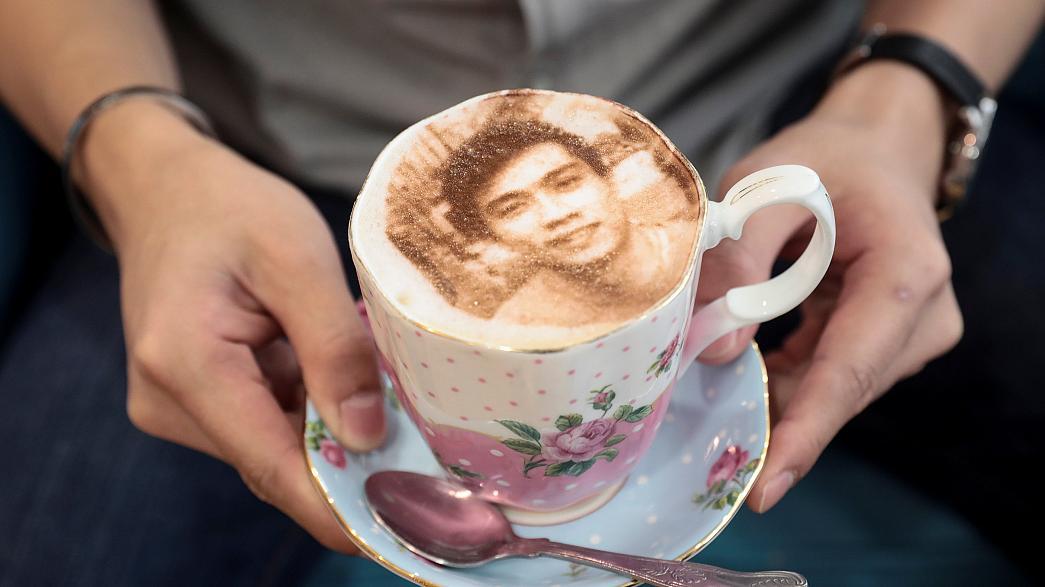
\includegraphics[scale=0.3]{slika_1}
\caption{\textit{Selfieccino} kafa}
\label{slika_1}
\end{figure}

Gosti putem aplikacije \v{s}alju svoju sliku ili neki tekst osoblju kafi\'ca koji onda za njih pripremaju ovaj neobi\v{c}ni napitak. Procedura izrade napitka traje \v{c}etiri minute, a cijena koju gosti trebaju platiti za ovo neobi\v{c}no pi\'ce je $5.75$ funti. Iako je cijena \textit{selfieccina} malo ve\'ca od prosje\v{c}ne cijene kafe, osoblje kafi\'ca je izjavilo da su prvi dan imali preko $400$ gostiju koji su tu do\v{s}li samo zbog ove inovacije.

Ideja za ovakav pristup pripremi kafe, prema rije\v{c}ima vlasnika kafi\'ca, je bila \v{z}elja da se spoje dvije itekako popularne stvari u \v{z}ivotu mladih - kafa i \textit{selfie}. Slično grčkom mitu o Narcissusu, čovjeku koji je bio tako uznemiren kada je vidio svoj odraz u jezeru da se odmah zaljubio, \textit{selfieccino} gostima omogućava da gledaju svoje lice dok ispijaju svoj omiljeni topli napitak \cite{bustle}. Vlasnik kafi\'ca, Ehab Salem Shouly, je izjavio za Reuters: "Nije dovoljno samo pružiti sjajnu hranu i odličnu uslugu - to mora biti vrijedno Instagrama". Ova izjava je autore ovog rada motivisala da probaju istu ideju implementirati na svoj na\v{c}in i u svom gradu. 

\newpage

\section{Konceptualni dizajn}

Konceptualni dizajn predstavlja prvi korak u procesu dizajna i razvoja sistema. U ovoj fazi se vrši identifikacija potreba, definišu se zahtjevi za potencijalno rješenje, zatim se potencijalna rješenja ocjenjuju i na osnovu toga se razvija specifikacija sistema. Specifikacija sistema predstavlja tehničke zahtjeve koji u potpunosti utiču na daljnji tok dizajna sistema. Kako ovaj dokument određuje cjelokupni budući razvoj, navedena faza ne može biti završena sve dok se ne utvrdi da specifikacije sistema adekvatno adresiraju identifikovane potrebe.

Klju\v{c}ni koraci u procesu konceptualnog dizajna su:
\begin{itemize}
\item identifikacija potreba,
\item analiza izvodljivosti,
\item analiza zahtjeva za sistem,
\item specifikacija sistema,
\item pregled idejnog rje\v{s}enja. \cite{wiki1}
\end{itemize}

Neka od pitanja koja mogu biti korisna u fazi konceptualnog dizajna su:
\begin{itemize}
\item Koliko truda treba ulo\v{z}iti u idejno rje\v{s}enje?
\item Koji koncept treba da bude osnova dizajna? 
\item Koju tehnologiju za dati podsistem treba odabrati?
\item Koji postoje\'ci hardver i softver treba koristiti?
\item Da li je predvi\dj eni koncept tehni\v{c}ki izvodi na osnovu tro\v{s}kova, rasporeda i performanse?
\item Da li su potrebna dodatna istra\v{z}ivanja prije nego se donese kona\v{c}na odluka? \cite{book1}
\end{itemize}

Za potrebe izrade seminarskog rada odabran je printer \textit{selfieccina}. U narednim poglavljima će biti opisane detaljne faze u okviru konceptualnog dizajna za predloženi sistem.

\newpage

\subsection{Identifikacija potreba}

Prema definiciji Oxfordovog rječnika engleskog jezika, selfie je fotografija gdje mi uslikamo samog sebe, najčešće koristeći pametni telefon ili web kameru kako bi podijelili tu fotografiju na društvenim medijima. Mada je sada rano praviti prognoze, selfie će ostaviti veliki trag na kulturu ljudi 21. vijeka i bit će zapamćen kao kulturološki fenomen našeg doba. 

Velikoj većini omladine, selfiji su postali svakodnevnica, te mnogo branše industrije to gledaju da iskoriste. Npr. postojanje prednje kamere na pametnim telefonima i njen kvalitet je direktno uslovljeno kulturom selfija, tj. selfiji su imali ogroman uticaj na razvoj današnjih pametnih telefona. Također mnoge kompanije gledaju da iskoriste selfije u svojim reklamnim kampanjama kako bi svoje proizvode približili omladini. 

Jedan od uređaja koji želi da iskoristi popularnost selfija jeste "Selfie Coffee Printer" koji trenutno proizvodi kompanije Cino iz Kine. Uređaj može da isprinta bilo koju fotografiju na površinu kafe (pa time i selfije). Na taj način nastaje takozvani "Selfieccino". 

Prateći novinske članke, što se tiče Europe, jedino je kafić u Londonu kupio tu mašinu, te prema tvrdnjama vlasnika prvi dan je kafić posjetilo 400 mušterija samo kako bi probali selfieccino i podijelili svoje selfie sa selficcinom na društvenim mre\v{z}ama. Očigledno, jedna takva mašina, osim što daje besplatnu promociju kafiću, povećava mu i profit, barem u prvom periodu dok je taj proizvod još svjež.

Tu mi vidimo priliku za mogući profit. Smatramo da bi bilo moguće napraviti "Selfie Coffee Printer" (u nastavku SCP) jeftiniji od trenutnog na tržištu, te ga uspješno prodati kafićima u našem regionu.

\subsection{Analiza izvodljivosti}
SCP se sastoji iz dva dijela:
\begin{enumerate}
\item Mehanizma za pomjeranje vrha za printanje
\item Vrh za printanje
\item Tinta za printanje
\end{enumerate}

\newpage

\subsubsection{Mehanizma za pomjeranje vrha za printanje}
Zadatak mehanizma jeste da pozicionira vrh za printanje na potrebnu poziciju kod površine kafe. Mehanizam mora biti dovoljno precizan da može isprintati svaki piksel slike na kafi za zadatu rezoluciju. Jedino rješenje koje se nameće jeste pravljenje mehanizma na isti način kao što 3D printeri imaju mehanizam za printanje, tj. korištenje 3 steper motora za svaku dimenziju prostora. Mada treća dimenzija možda izgleda suvišno, dodavanjem treće dimenzije moguće bi bilo printati za razne profile čaša za kafu.

\subsubsection{Vrh za printanje}
Kod vrha za printanje postoji nekoliko mogućih alternativa:
\begin{itemize}
\item šprice,
\item inkjet tehnologija,
\item airbrush.
\end{itemize}

Prva alternativa jeste korištenje šprica sličnih kao što se koriste u medicni za ispuštanje boje na površinu kafe. Intuicijom, a i testiranjem te metode je pokazano da su početne kapljice prevelike da budu korisne u printanju.

Druga alternativa jeste korištenje postojećih inkjet tehnologija uz jestivu tintu za printanje po površini kafe. Međutim, programiranje inkjet tonera kada da ispuštaju tintu ili rastavljanje postojećih printera kako bi se koristila njihova tehnologija ne predstavlja dobru opciju zbog velikih troškova kupovine printera i velike ovisnosti od softvera proizvođača printera.

Zadnja alternativa izgleda najisplativija, tj. korištenje airbrush tehnologije za ispuštanje malih količina tinte. 

\subsubsection{Tinta za printanje}

Glavni uslov za tintu jeste da mora biti jestiva. Pošto će se koristiti airbursh tehnologija, potencijalno se može koristiti i suha tinta, tj. recimo sitno samljevena zrna kafe. Na taj način korisnici ne bi morali kupovati dodatnu tintu nakon kupovine proizvoda što je veliki plus za ukupni proizvod. Odluka o tome koja vrsta tinte će se koristiti će biti donesena u sljedećim fazama razvoja proizvoda, kada se analiziraju obje vrste tinte.

\newpage

\subsection{Analiza zahtjeva za sistem}
\subsubsection{Operativni zahtjevi}

\textbf{Gdje će se sistem koristiti?}\\
Sistem će se koristiti u ugostiteljskim objektima. 

\textbf{Šta sistem treba da ostvari i koje funkcije da primjeni kako bi zadovoljio potrebe?}\\
Kako bi ostvario već ranije definisane potrebe, sistem treba biti jeftiniji od već postojećih sistema.

\textbf{Koji su to kritični sistemski parametri potrebni za ostvarenje misije?}\\
Kritični parametri koji definišu SCP su:
\begin{itemize}
\item Vrijeme printanja
\item Rezolucija
\item Preciznost
\end{itemize}

\textbf{U kojoj mjeri će sistem biti korišten?}\\
Kako bi se sistem koristio u kafićima treba biti sposoban da radi svih 7 dana u sedmici, sa prosječnim brojem od 100 isprintanih kafa po danu.

\textbf{Koliko efikasan sistem mora biti?}\\
Najbitniji parametri vezani za efikasnost su srednje vrijeme između kvarova (MTBF), srednje vrijeme perioda dok je sistem izvan funkcije (MDT) i srednje vrijeme između održavanja (MTBM). U nastavku će ovi parametri biti bolje definisani.

\textbf{Koliko dugo će korisnik koristiti sistem?}\\
Kako bi sistem bio primamljiv za kupovinu, potrebno je da se može koristiti barem godinu dana (tj. da garancija traje godinu dana).

\textbf{Koji su zahtjevi na okolinu u kojoj će sistem operisati?}\\
Pošto će se ovaj sistem koristi u ugostiteljskim objektima gdje se temperatura održava u ugodnom opsegu od 15°C do 25°C, to je također i temperaturni opseg u kojem treba da funkcioniše i sistem.

\newpage

\subsection{Zahtjevi za održavanje i podršku}
\textbf{Gdje će se raditi, na koji način i ko će biti odgovaran za održavanje i popravka sistema?}\\
Sistem će se popravljati i održavati na mjestu gdje se i koristi, te će proizvođač biti odgovoran za popravku.
%te će popratna dokumentacija kao i jednostavnost sistema omogućiti to da sami korisnik može raditi popravku sistema.

\textbf{Kakve usluge popravke i podrške će pružati proizvođač?}\\
U slučaju kvarova, proizvođač će ili popravljati pokvarene komponente ili ih potpuno mijenjati. 
%zbog modularnosti sistema, proizvođač će poslati zamjenske module kako bi se popravio kvar.  

\subsection{Dodatni zahtjevi}
Pored prethodno pomenutih zahtijeva u ovom poglavlju \'ce biti opisani dodatni zahtijevi koji \'ce biti smjernice prilikom dizajna sistema printera \textit{selfieccina}. Koliko god obra\'cali pa\v{z}nju na performanse sistema, implementaciju efikasnih algoritama za pretvaranje slike u koordinate za printanje kontura lica, optimizaciju kretanja vrha printera potrebno je obratiti pa\v{z}nju na zahtijeve koji su veoma bitni krajnjim korisnicima proizvoda, tj. onima koji ne znaju i koje ne zanima \v{s}ta se to de\v{s}ava unutar printera i mikrokontrolera koji njime upravlja ve\'c ono \v{s}to je vidljivo ljudskom oku i \v{s}to \v{c}ini kupce zadovoljnim.

Neki od tih zahtijeva su:
\begin{itemize}
\item lijep i modernisti\v{c}ki dizajn printera,
\item brzina izrade napitka,
\item preciznost u printanju slike,
\item niska cijena.
\end{itemize}

Koliko god dobar algoritam bio u pozadini printera, ono \v{s}to u kona\v{c}nici predstavlja jedan od najbitnijih faktora za prodaju proizvoda je lijep i modernisti\v{c}ki dizajn. Vlasnici kafi\'ca, koji su potencijalni kupci printera, moraju ste\'ci dojam da je printer adekvatan za prostoriju u kojoj ga planiraju koristiti. Printer treba imati takav dizajn da se uklapa u interijer svih objekata u kojima bi se trebao koristiti, jer i pored toga \v{s}to je proces pripremanja ovog neobi\v{c}nog napitka itekako zanimljiv bitan je vanjski izgled koji \'ce dodatno uticati na faktor odu\v{s}evljenja.

\newpage

Vrijeme je novac, izreka je koja je motivacija za postizanje \v{s}to ve\'ce brzine izrade napitka. Ovo je veoma bitan faktor ovog sistema, jer u dana\v{s}njem veoma dinami\v{c}nom na\v{c}inu \v{z}ivota vlasnik kafi\'ca ne \v{z}eli da korisnici moraju potro\v{s}iti puno vremena \v{c}ekaju\'ci svoj \textit{selfieccino} jer i pored svega to je ipak samo obi\v{c}na kafa.

Preciznost u printanju slike predstavlja jedan od najbitnijih zahtijeva u dizajnu ovog sistema. Ciljno tr\v{z}i\v{s}te ovog sistema su korisnici koji \'ce namjenski dolaziti u kafi\'c sa \textit{selfieccino} printerom i ba\v{s} zbog toga treba se potruditi da dobiju ono zbog \v{c}ega su i do\v{s}li, kvalitetno isprintan \textit{selfie} na pjeni njihovog toplog napitka.

Cijena, kao i u svakom drugom segmentu poslovnog \v{z}ivota, predstavlja jedan od bitnih faktora u dizajnu sistema. Niska cijena printera  ali i samog procesa izrade \textit{selfieccina} je faktor koji \'ce znatno olak\v{s}ati proces komercijalizacije sistema, te zbog toga \'ce ovaj zahtijev biti jedna od glavnih vodilja prilikom procesa dizajna i izrade printera.
 
\subsection{Tehni\v{c}ke mjere performanse} 

Prilikom dizajna proizvoda, veoma bitan korak predstavlja i odgovaraju\'ca metrika koja opisuje sistem koji se dizajnira. Ovu metriku mo\v{z}emo zamisliti kao kvantitativni faktor koji dodjeljuje odgovaraju\'cu ocjenu odre\dj enom dizajnu sistema, te se na osnovu njega mogu porediti razli\v{c}iti dizajni. Prethodno pomenute metrike se jo\v{s} nazivaju i \textit{tehni\v{c}ke mjere performanse} (\textbf{eng} Technical performance measures (TPMs)). Njihova primjena vodi do identifikacije parametara neophodnih za dizajn sistema i realizaciju \v{z}eljenih funkcionalnosti. Kako bi se prilikom dizajna sistema vodili ovim metrikama, potrebno ih je definisati na po\v{c}etku samog procesa. 

Veoma bitan faktor prilikom dizajna metrike koja \'ce dati ocjenu za dizajnirani sistem je odre\dj ivanje te\v{z}inskih koeficijenata za pojedina\v{c}ne zahtjeve. To \'ce omogu\'citi lak\v{s}u komunikaciju izme\dj u krajnjeg korisnika i onoga ko dizajnira dati sistem. Veoma popularna tehnika koja omogu\'cava uva\v{z}avanje korisni\v{c}kih zahtjeva pri dizajnu sistema je QFD (\textbf{eng} Quality Function Deployment) tehnika. Ideja QFD tehnike je identificirati neophodne zahtjeve i prevesti ih u tehni\v{c}ka rje\v{s}enja. Korisni\v{c}kim zahtijevima se dodijeljuju te\v{z}inski faktori na osnovu stepena prioriteta svakog od njih. QFD metoda omogu\'cava dizajneru da bolje razumije korisni\v{c}ke zahtijeve, ali isto tako forsira korisnika da klasificira svoje zahtijeve prema njihovoj va\v{z}nosti. Klasifikacija zahtijeva prema njihovoj va\v{z}nosti omogu\'cava dizajneru i korisniku da porede razli\v{c}ite dizajne sistema. Svaki od korisni\v{c}kih zahtijeva se mora realizirati odre\dj enim tehni\v{c}kim rje\v{s}enjem. 

\newpage

QFD proces podrazumijeva formiranje jedne ili vi\v{s}e matrica koje povezuju razli\v{c}ite potrebe i zahtijeve koje je potrebno uva\v{z}iti prilikom dizajna. Jedna od prethodno pomenutih matrica je i \textit{House of Quality} (HOQ) matrica, koja je prikazana na slici \ref{hoq}.  

\begin{figure}[!h]
\centering
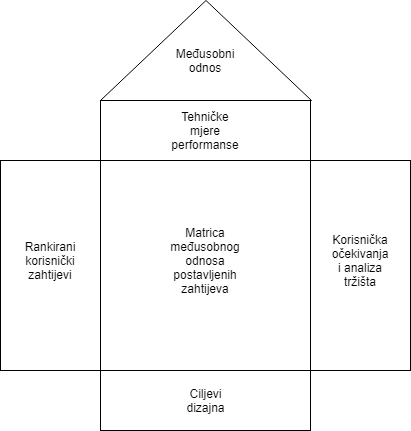
\includegraphics[scale=0.8]{hoq}
\caption{\textit{House of quality}}
\label{hoq}
\end{figure}
 
Kako bi se konstruisala uspje\v{s}na \textit{House of Quality}, koja bi olak\v{s}ala proceduru dizajna sistema veoma je bitno dobro definisati zahtijeve i njihove prioritete u po\v{c}etnoj fazi. Na ovaj na\v{c}in se dobija i veoma dobar pregled svih zahtijeva i njihovih tehni\v{c}kih rje\v{s}enja. Tehni\v{c}ke mjere performanse predstavljaju jedan od najbitnijh faktora. One predstavljaju odgovaraju\'cu metriku koja ocjenjuje stepen va\v{z}nosti pojedina\v{c}nih zahtijeva i na taj na\v{c}in predstavlja vodi\v{c} za dizajnera sistema. Izgled House of Quality-a, kao rankirane tehni\v{c}ke mjere performanse za sistem \textit{Selfieccino} su prikazani na sljede\'cim tabelama. 

U tabeli \ref{tabela ponudjenih rjesenja} se mogu vidjeti ponuđena tehnička rješenja koja su dobivena kao rezultat HoQ analize te FMECA analize iz narednog poglavlja. Nakon što se uradi analiza dizajna za pouzdanost, održivost i Life-cyle cost, bit će moguće odabrati koje od ponuđenih rješenja je najisplativije, te time i rješenje koje treba odabrati. 
\begin{table}
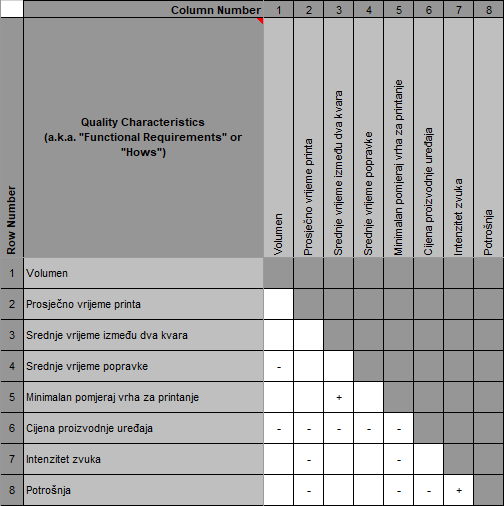
\includegraphics[scale=1]{tabela_gornja}
\caption{Tabela tehničke korelacije}
\end{table}


\begin{table}
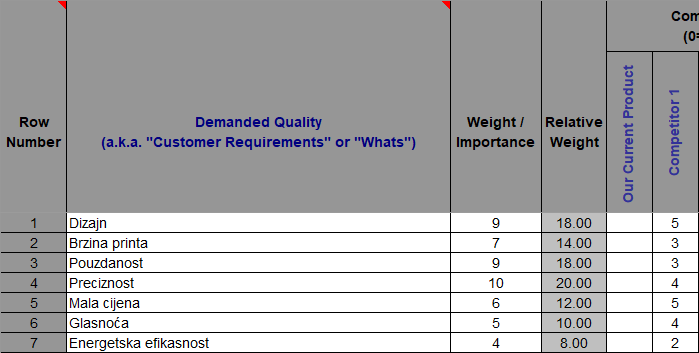
\includegraphics[width=\textwidth]{tabela_zahtjevi_korisnika}
\caption{Tabela zahtjeva korisnika}
\end{table}

\begin{table}
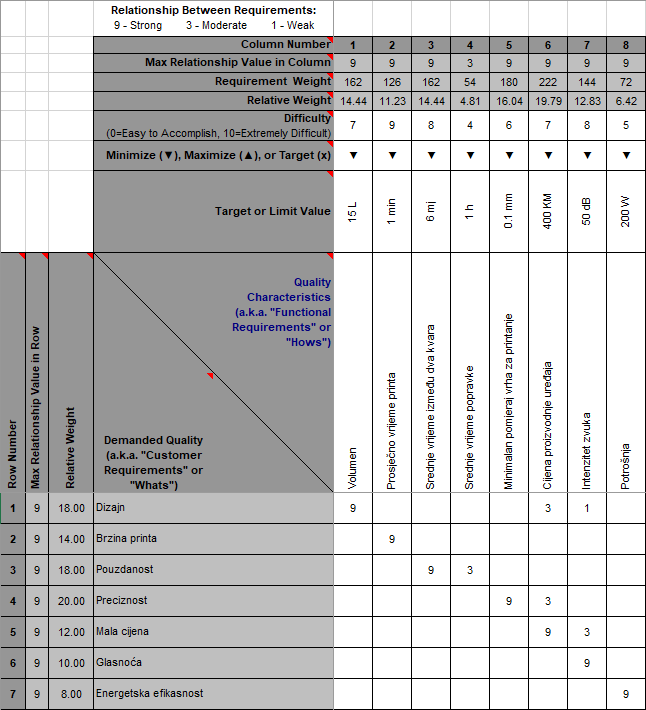
\includegraphics[width=\textwidth]{tabela_sredina}
\caption{Tabela veze između korisničkih i tehničkih zahtjeva}
\end{table}

\begin{table}
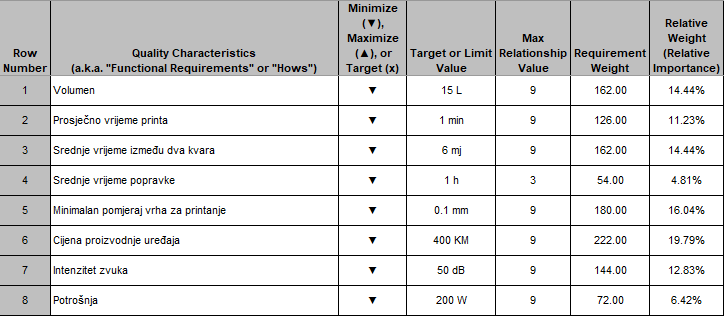
\includegraphics[width=\textwidth]{tabela_zakljucak}
\caption{Tabela ocjene dizajna tehničkih mjerila}
\end{table}

\begin{table}
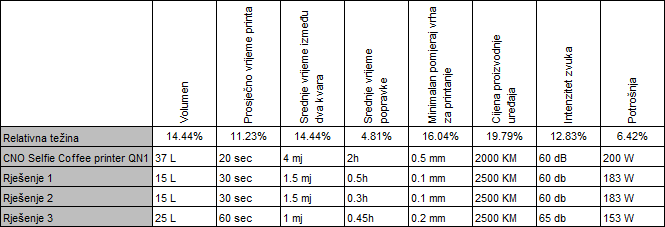
\includegraphics[width=\textwidth]{tabela_donja}
\caption{Tabela ponuđenih tehničkih rješenja}
\label{tabela ponudjenih rjesenja}
\end{table}

\clearpage


\subsection{Funkcionalna analiza i alokacija}
\subsubsection{Funkcionalna analiza}
Funkcionalna analiza predstavlja proces prevo\dj enja zahtijeva u kriterij za dizajn sistema uz identifikaciju specifi\v{c}nih zahtijeva za potrebnim resursima. Analiza zapo\v{c}inje sa korisni\v{c}kim zahtijevima a zavr\v{s}ava sa identificiranim zahtijevima za hardver, softver i sve ostale neophodne resurse.

Funkcionalna analiza zapo\v{c}inje definisanjem funkcionalnosti koje sistem treba da ispunjava. Ideja je da se ta\v{c}no defini\v{s}e \textbf{\v{s}ta} se treba uraditi, a ne \textbf{kako} to treba uraditi. Nijedan dio opreme, hardvera, softvera, ljudstva i bilo kojeg drugog resursa ne bi trebao biti kupljen ili planiran sve dok se funkcionalna analiza sistema ne provede do kraja. Funkcionalna analiza je iterativna procedura tokom koje se ve\'ci zahtijevi razbijaju na manje. Ova dekompozicija se obavlja sve dok se ne do\dj e do najni\v{z}eg nivoa na kojem je mogu\'ce identificirati resurse potrebne za ispunjavanje date funkcionalnosti. Za ove potrebe se koriste funkcionalni dijagrami. Oni omogu\'cavaju razbijanje funkcionalnosti sistema na manje dijelove i dobru vizuelnu reprezentaciju istih. 

Funkcionalni dijagram sistema \textit{Selfieccino} je prikazan na slici \ref{funkcdijagram}. 

\subsubsection{Funkcionalna alokacija}
Nakon definisanja funkcionalnog dijagrama \textit{selfieccina}, sljede\'ci korak je grupisanje malih funkcionalnosti u logi\v{c}ke blokove. Na ovaj na\v{c}in \'ce se izvr\v{s}iti identifikacija svih podsistema koje je potrebno implementirati u sklopu cijelog sistema. U ovom koraku se dekompozicija iz prethodnog poglavlja, koja se bavila pitanjem \textit{\v{s}ta} treba implementirati, prevodi u formu \textit{kako} to treba implementirati. Ovakva dekompozicija sistema \textit{selfieccina} je prikazana na slici \ref{funkcalokacija}.

\newpage

\begin{figure}[!h]
\centering
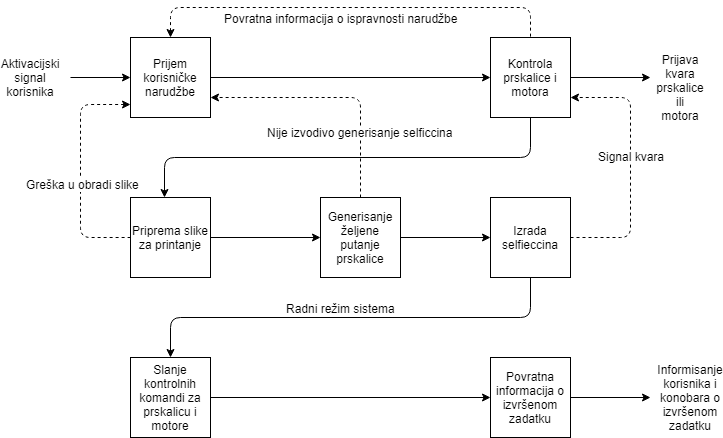
\includegraphics[scale=0.65]{funkcdijagram}
\caption{Funkcionalni dijagram \textit{selfieccina}}
\label{funkcdijagram}
\end{figure}

\newpage

\begin{figure}[!h]
\centering
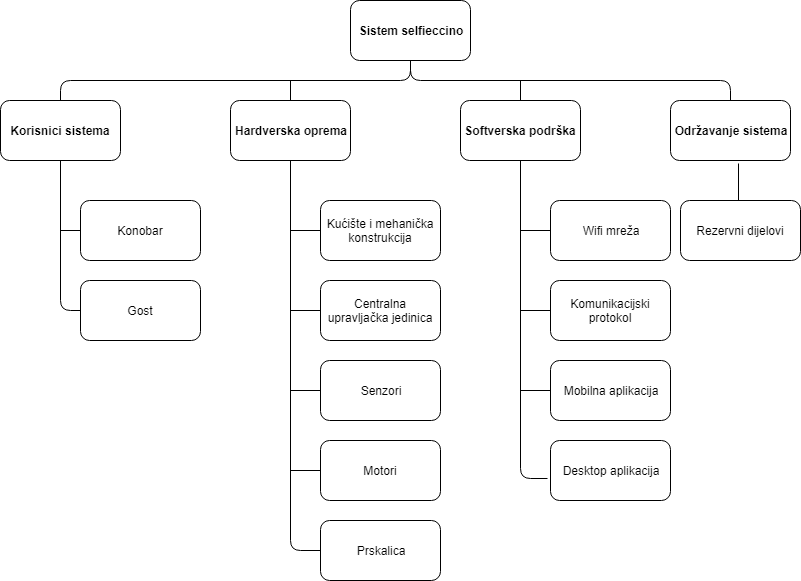
\includegraphics[scale=0.6]{funkcalokacija}
\caption{Funkcionalna alokacija \textit{selfieccina}}
\label{funkcalokacija}
\end{figure}
 
 \newpage
\subsection{FMECA analiza} 
FMECA (\textbf{eng} Failure Mode, Effects and Criticality Analysis) predstavlja tehniku analize koja se koristi za istra\v{z}ivanje i identifikaciju potencijalnih slabosti sistema \cite{oakes1}. Primjena ove tehnike omogu\'cava da se provede analiza koja \'ce ispitati sve mogu\'ce kvarove sistema, uticaj tih kvarova na rad, sigurnost i performanse sistema.

Kako se sistem \textit{selfieccina} mo\v{z}e konceptualno razdvojiti na fizi\v{c}ki i funkcionalni dio, FMECA analiza \'ce biti provedena na oba dijela sistema. FMECA analiza se sastoji od 12 klj\v{c}nih koraka (detaljno opisano u radu \cite{oakes1}). U sljede\'cim tabelama \'ce biti detaljno provedena FMECA analiza fizi\v{c}kog i funkcionalnog dijela sistema.

\newpage

\begin{table}[!h]
\begin{tabular}{|p{25mm}|p{25mm}|p{25mm}|p{25mm}|p{25mm}|}
\hline 
\textbf{Fizi\v{c}ka komponenta} & \textbf{Potencijalni kvar} & \textbf{Potencijalni uzrok kvara} & \textbf{Potencijalni uticaj kvara na proizvo\dj a\v{c}a} & \textbf{Potencijalni uticaj kvara na korisnika} \\ 
\hline 
\textbf{Ku\'ci\v{s}te i mehani\v{c}ka konstrukcija} & Fizi\v{c}ka o\v{s}te\'cenja & Udarci o\v{s}trim predmetima & Naru\v{s}avanje estetike & Naru\v{s}avanje estetike  \\ 
\hline
\textbf{Upravlja\v{c}ka jedinica} & Kvar elektroni\v{c}kih komponenti & Prekid napajanja & Dodatni tro\v{s}kovi & Nezadovoljstvo pru\v{z}enom uslugom \\ 
\hline
\textbf{Senzor udaljenosti} & Pogre\v{s}na o\v{c}itanja senzora & Lo\v{s}a kalibracija senzora & Lo\v{s} kvalitet proizvoda & Nezadovoljstvo pru\v{z}enom uslugom \\ 
\hline
\textbf{Motori} & Prestanak rada, pogr\v{s}na veli\v{c}ina koraka & Prestanak napajanja, lo\v{s}a kalibracija, lo\v{s}e generisana putanja kretanja & Lo\v{s} kvalitet proizvoda & Nezadovoljstvo pru\v{z}enom uslugom \\ 
\hline
\textbf{Prskalica} & Prestanak rada, gre\v{s}ka u koli\v{c}ini materije koja se izbacuje & Prestanak napajanja, fizi\v{c}ko o\v{s}te\'cenje komponenti prskalice & Lo\v{s} kvalitet proizvoda & Nezadovoljstvo pru\v{z}enom uslugom \\ 
\hline 
\end{tabular}
\caption{FMECA analiza fizi\v{c}kih komponenti (prvi dio tabele)}
\end{table}
 
 \newpage
 
\begin{table}[!h]
\begin{tabular}{|p{25mm}|p{25mm}|p{25mm}|p{25mm}|p{25mm}|}
\hline 
\textbf{Metod detekcije kvara} & \textbf{Ozbiljnost kvara} & \textbf{U\v{c}estalost kvara} & \textbf{Vjerovatno\'ca otkrivanja kvara} & \textbf{Prioritet opasnosti RPN} \\ 
\hline 
Vizuelno & 3 & 2 & 9 & 54 \\ 
\hline 
Mjerenje struje, napona i temperature i vizuelna analiza funkcionalnosti sistema & 10 & 4 & 8 & 320 \\
\hline
Mjerenje struje, napona i analiza povratnih informacija sa senzora & 10 & 3 & 7 & 210 \\
\hline
Vizuelno & 9 & 3 & 10 & 270 \\
\hline
Vizuelno & 9 & 4 & 8 & 288 \\
\hline
\end{tabular}
\caption{FMECA analiza fizi\v{c}kih komponenti (drugi dio tabele)}
\end{table}

\newpage

\begin{table}[!h]
\begin{tabular}{|p{25mm}|p{25mm}|p{25mm}|p{25mm}|p{25mm}|}
\hline 
\textbf{Funkcionalna komponenta} & \textbf{Potencijalni kvar} & \textbf{Potencijalni uzrok kvara} & \textbf{Potencijalni uticaj kvara na proizvo\dj a\v{c}a} & \textbf{Potencijalni uticaj kvara na korisnika} \\ 
\hline 
\textbf{Wifi mre\v{z}a} & Nestanak konekcije & Gre\v{s}ka na strani internet provajera, preoptere\'cenje mre\v{z}e & Ka\v{s}njenje u proizvodnji & Nezadovoljstvo pru\v{z}enom uslugom  \\ 
\hline
\textbf{Komunikac. protokol} & Zagu\v{s}enje komunikacijskog kanala & Lo\v{s}a kontrola pristupa ure\dj aju & Ka\v{s}njenje u proizvodnji & Nezadovoljstvo pru\v{z}enom uslugom \\ 
\hline
\textbf{Mobilna aplikacija} & Prestanak rada aplikacije & Neotkrivene gre\v{s}ke u implementaciji aplikacije & Lo\v{s} kvalitet pru\v{z}anja usluga & Nezadovoljstvo pru\v{z}enom uslugom \\ 
\hline
\textbf{Desktop aplikacija} & Prestanak rada aplikacije & Neotkrivene gre\v{s}ke u implementaciji aplikacije & Lo\v{s} kvalitet pru\v{z}anja usluga & Nezadovoljstvo pru\v{z}enom uslugom \\ 
\hline 
\end{tabular}
\caption{FMECA analiza funkcionalnih komponenti (prvi dio tabele)}
\end{table}

\newpage

\begin{table}[!h]
\begin{tabular}{|p{25mm}|p{25mm}|p{25mm}|p{25mm}|p{25mm}|}
\hline 
\textbf{Metod detekcije kvara} & \textbf{Ozbiljnost kvara} & \textbf{U\v{c}estalost kvara} & \textbf{Vjerovatno\'ca otkrivanja kvara} & \textbf{Prioritet opasnosti RPN} \\ 
\hline 
Gubitak konekcije ure\dj aja & 5 & 5 & 10 & 250 \\ 
\hline 
Pogre\v{s}an format primljenih podataka & 7 & 4 & 8 & 224 \\
\hline
Prijava od strane korisnika & 7 & 4 & 9 & 252 \\
\hline
Prijava od strane konobara & 8 & 2 & 10 & 160 \\
\hline
\end{tabular}
\caption{FMECA analiza funkcionalnih komponenti (drugi dio tabele)}
\end{table}

\newpage


Na slici \ref{fmeca} je prikazan RPN za funkcionalne i fizi\v{c}ke komponente sistema.

\begin{figure}[!h]
\centering
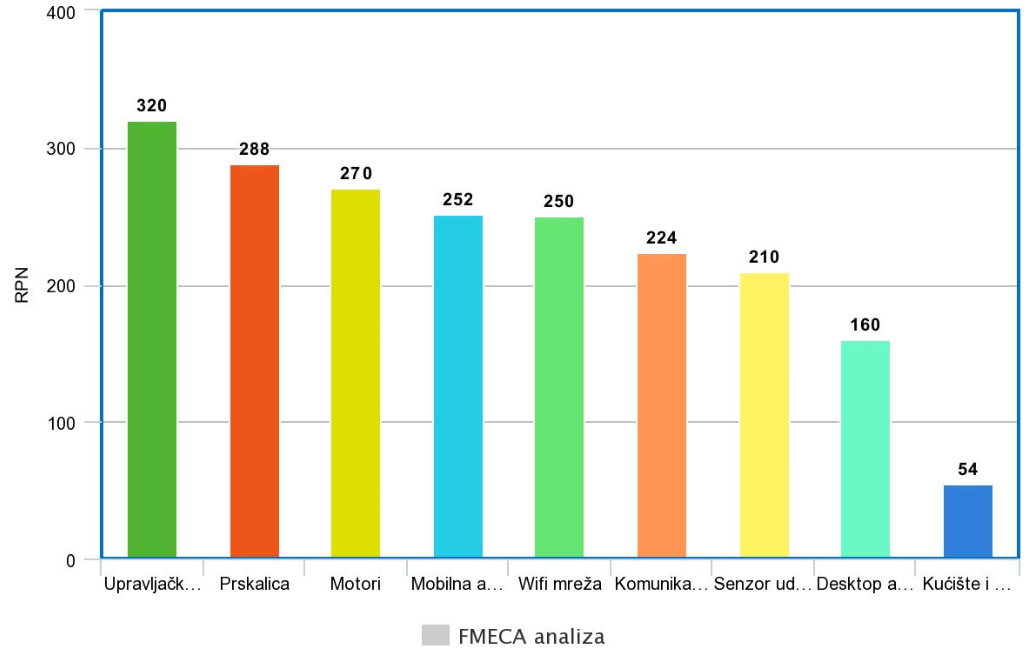
\includegraphics[scale=0.6]{fmeca}
\caption{Grafi\v{c}ki prikaz RPN-a}
\label{fmeca}
\end{figure}

Kako bi se smanjile vrijednosti RPN-a, mogu\'ce je uvesti neke dodatne preporuke koje su prikazane u sljede\'coj tabeli.

\newpage

\begin{table}[!h]
\begin{tabular}{|p{25mm}|p{25mm}|p{25mm}|p{25mm}|p{25mm}|p{25mm}|}
\hline 
\textbf{Komponenta} & \textbf{Preporuka za pobolj\v{s}anje} & \textbf{Ozbiljnost kvara} & \textbf{U\v{c}estalost kvara} & \textbf{Vjerovatno\'ca otkrivanja kvara} & \textbf{Prioritet opasnosti RPN} \\ 
\hline 
Ku\'ci\v{s}te i mehani\v{c}ka konstrukcija & Kvalitetniji materijal & 2 & 1 & 7 & 14 \\ 
\hline 
Upravlja\v{c}ka jedinica & Bolji mikrokontroler & 10 & 2 & 7 & 140 \\
\hline
Senzor udaljenosti & Dodatni senzori udaljenosti, laserski senzori & 10 & 1 & 6 & 60 \\
\hline
Motori & Kvalitetniji motori sa zasebnim drajverima & 8 & 2 & 5 & 80 \\
\hline
Prskalica & Profesionalno izra\dj ena prskalica & 8 & 2 & 7 & 112 \\
\hline
Wifi mre\v{z}a & Skalabilna mre\v{z}a i dobar internet provajder & 5 & 2 & 8 & 80 \\
\hline
Komunikac. protokol & Sigurniji i pouzdaniji implementirani protokol & 5 & 2 & 7 & 70 \\
\hline
Mobilna aplikacija & Profesionalni developeri za razvoj aplikacije & 5 & 2 & 8 & 80 \\
\hline
Desktop aplikacija & Profesionalni developeri za razvoj aplikacije & 5 & 2 & 5 & 50 \\
\hline
\end{tabular}
\caption{Preporuke za pobolj\v{s}anje RPN-a}
\end{table}

\newpage

Na slici \ref{fmeca2} je prikazana pobolj\v{s}ana verzija RPN-a za funkcionalne i fizi\v{c}ke komponente sistema.

\begin{figure}[!h]
\centering
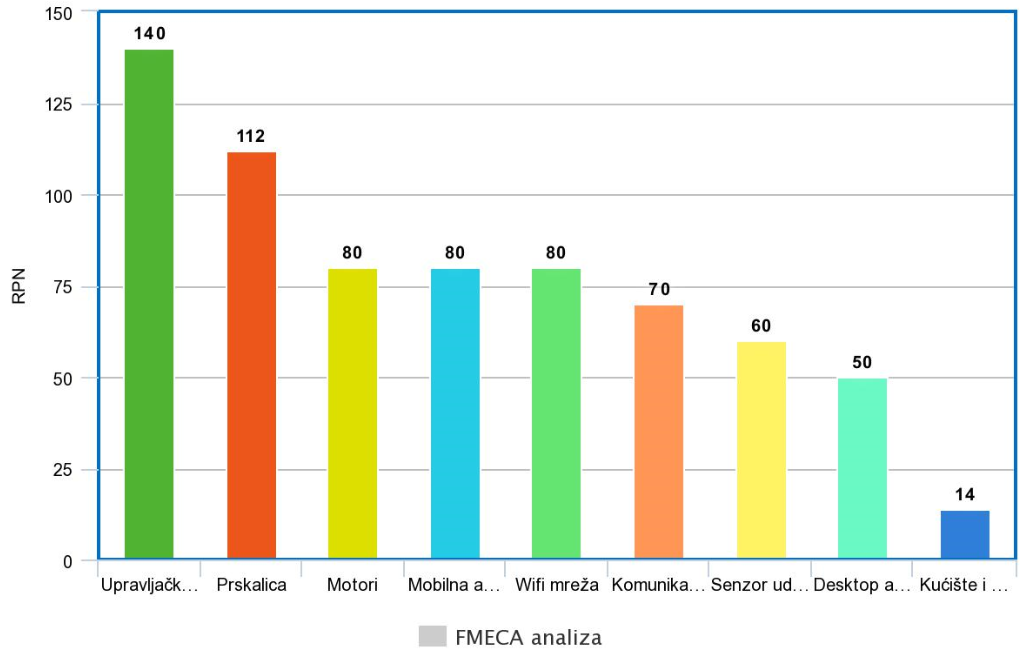
\includegraphics[scale=0.6]{fmecaBolji}
\caption{Grafi\v{c}ki prikaz RPN-a sa preporu\v{c}enim akcijama za pobolj\v{s}anje}
\label{fmeca2}
\end{figure}

\subsection{Predložena rješenja i alokacija zahtjeva}

Na osnovu zahtjeva, HoQ i FMECA analiza, predložena su tri moguća rješenja koja se vide na tabelama \ref{tab:rjesenje1}, \ref{tab:rjesenje2} i \ref{tab:rjesenje3}. Prvo rješenje predstavlja mali i brzi printer koji bi bio idealan proizvod za kupce. Drugi proizvod ima slične karakteristike kao prvi. Jedina razlika je u tome što ima veći volumen koji smanjuje vrijeme popravke jer je pristup komponentama olakšan. Treće rješenje je slično kao drugo, ali je razlika u korištenju jeftinijih motora kako bi se smanjila cijena proizvodnje. To zauzvrat ima posljedicu smanjenje srednjeg vremena između dva kvara.

Kao što se može vidjeti u tabelama je urađena također i alokacija zahtjeva za srednje vrijeme između dva kvara kao i  srednjeg vremena popravke koje predstavljaju dijelove dizajna za pouzdanost i održivost.
\begin{landscape}


\begin{table}[]
\scriptsize
  \centering
  \caption{Alokacija zahtjeva: Rješenje 1 (Mal volumen, precizan, brz i tih print)}
    \begin{tabular}{ccccccccc}

    \midrule
    Cjelina & Komponente & Broj jedinica & MTBF(h) & \multicolumn{1}{p{5.215em}}{Doproinos\newline{}kvarovima} & Mct(h) & Cijena(KM) & Potrošnja (W) & Intenzitet zvuka (db) \\
    \midrule
    \multirow{2}[4]{*}{Upravljačka jedinica} & \multicolumn{1}{l}{Driver za motore} & \multicolumn{1}{r}{1} & \multicolumn{1}{r}{2500} & \multicolumn{1}{r}{11.48\%} & \multicolumn{1}{r}{0.3} & \multicolumn{1}{r}{20} & \multicolumn{1}{r}{5} &  \\
\cmidrule{5-5}          & \multicolumn{1}{l}{Mikrokontroler} & \multicolumn{1}{r}{1} & \multicolumn{1}{r}{2500} & \multicolumn{1}{r}{11.48\%} & \multicolumn{1}{r}{0.3} & \multicolumn{1}{r}{10} & \multicolumn{1}{r}{1} &  \\
    \midrule
    \multirow{4}[8]{*}{Mehanizam printanja} & \multicolumn{1}{l}{Motori} & \multicolumn{1}{r}{3} & \multicolumn{1}{r}{4000} & \multicolumn{1}{r}{7.18\%} & \multicolumn{1}{r}{2} & \multicolumn{1}{r}{250} & \multicolumn{1}{r}{170} & \multicolumn{1}{r}{50} \\
\cmidrule{5-5}          & \multicolumn{1}{l}{Okvir} & \multicolumn{1}{r}{1} & \multicolumn{1}{r}{10000} & \multicolumn{1}{r}{2.87\%} & \multicolumn{1}{r}{3} & \multicolumn{1}{r}{100} &       &  \\
\cmidrule{5-5}          & \multicolumn{1}{l}{Prskalica} & \multicolumn{1}{r}{1} & \multicolumn{1}{r}{2000} & \multicolumn{1}{r}{14.35\%} & \multicolumn{1}{r}{0.7} & \multicolumn{1}{r}{20} &       & \multicolumn{1}{r}{60} \\
\cmidrule{5-5}          & \multicolumn{1}{l}{Spremnik pritiska} & \multicolumn{1}{r}{1} & \multicolumn{1}{r}{3000} & \multicolumn{1}{r}{9.57\%} & \multicolumn{1}{r}{1} & \multicolumn{1}{r}{25} & \multicolumn{1}{r}{5} & \multicolumn{1}{r}{40} \\
    \midrule
    \multirow{2}[4]{*}{Komunikacija} & \multicolumn{1}{l}{Wifi modul za komunikaciju} & \multicolumn{1}{r}{1} & \multicolumn{1}{r}{2000} & \multicolumn{1}{r}{14.35\%} & \multicolumn{1}{r}{0.3} & \multicolumn{1}{r}{5} & \multicolumn{1}{r}{1} &  \\
\cmidrule{5-5}          & \multicolumn{1}{l}{USB modul za komunikaciju} & \multicolumn{1}{r}{1} & \multicolumn{1}{r}{2000} & \multicolumn{1}{r}{14.35\%} & \multicolumn{1}{r}{0.3} & \multicolumn{1}{r}{5} & \multicolumn{1}{r}{1} &  \\
    \midrule
          & \multicolumn{1}{l}{Ukupno:} &       & \multicolumn{1}{r}{287.0813} & \multicolumn{1}{r}{100\%} & \multicolumn{1}{r}{0.580861} & \multicolumn{1}{r}{435} & \multicolumn{1}{r}{183} & \multicolumn{1}{r}{60} \\
    \midrule
    \multicolumn{9}{c}{Dobiveno: Volumen 15 L, Prosječno vrijeme printa 30 sec, minimalan pomjeraj prskalice 0.1 mm} \\
    \bottomrule
    \end{tabular}%
  \label{tab:rjesenje1}%
\end{table}%

% Table generated by Excel2LaTeX from sheet 'Alokacija zahtjeva'
\begin{table}[htbp]
    \scriptsize
  \centering
  \caption{Alokacija zahtjeva: Rješenje 2 (Srednji volumen, precizan, brz i tih print)}
    \begin{tabular}{ccccccccc}

    \toprule
    \multicolumn{1}{l}{Cjelina} & \multicolumn{1}{l}{Komponente} & \multicolumn{1}{l}{Broj jedinica} & \multicolumn{1}{l}{MTBF(h)} & \multicolumn{1}{p{5.215em}}{Doproinos\newline{}kvarovima} & \multicolumn{1}{l}{Mct(h)} & \multicolumn{1}{l}{Cijena(KM)} & \multicolumn{1}{l}{Potrošnja (W)} & \multicolumn{1}{l}{Intenzitet zvuka (db)} \\
    \midrule
    \multirow{2}[4]{*}{Upravljačka jedinica} & \multicolumn{1}{l}{Driver za motore} & \multicolumn{1}{r}{1} & \multicolumn{1}{r}{2500} & \multicolumn{1}{r}{11.48\%} & \multicolumn{1}{r}{0.1} & \multicolumn{1}{r}{20} & \multicolumn{1}{r}{5} &  \\
\cmidrule{5-5}          & \multicolumn{1}{l}{Mikrokontroler} & \multicolumn{1}{r}{1} & \multicolumn{1}{r}{2500} & \multicolumn{1}{r}{11.48\%} & \multicolumn{1}{r}{0.1} & \multicolumn{1}{r}{10} & \multicolumn{1}{r}{1} &  \\
    \midrule
    \multirow{4}[8]{*}{Mehanizam printanja} & \multicolumn{1}{l}{Motori} & \multicolumn{1}{r}{3} & \multicolumn{1}{r}{4000} & \multicolumn{1}{r}{7.18\%} & \multicolumn{1}{r}{1} & \multicolumn{1}{r}{250} & \multicolumn{1}{r}{170} & \multicolumn{1}{r}{50} \\
\cmidrule{5-5}          & \multicolumn{1}{l}{Okvir} & \multicolumn{1}{r}{1} & \multicolumn{1}{r}{10000} & \multicolumn{1}{r}{2.87\%} & \multicolumn{1}{r}{2} & \multicolumn{1}{r}{50} &       &  \\
\cmidrule{5-5}          & \multicolumn{1}{l}{Prskalica} & \multicolumn{1}{r}{1} & \multicolumn{1}{r}{2000} & \multicolumn{1}{r}{14.35\%} & \multicolumn{1}{r}{0.5} & \multicolumn{1}{r}{20} &       & \multicolumn{1}{r}{60} \\
\cmidrule{5-5}          & \multicolumn{1}{l}{Spremnik pritiska} & \multicolumn{1}{r}{1} & \multicolumn{1}{r}{3000} & \multicolumn{1}{r}{9.57\%} & \multicolumn{1}{r}{0.5} & \multicolumn{1}{r}{25} & \multicolumn{1}{r}{5} & \multicolumn{1}{r}{40} \\
    \midrule
    \multirow{2}[4]{*}{Komunikacija} & \multicolumn{1}{l}{Wifi modul za komunikaciju} & \multicolumn{1}{r}{1} & \multicolumn{1}{r}{2000} & \multicolumn{1}{r}{14.35\%} & \multicolumn{1}{r}{0.1} & \multicolumn{1}{r}{5} & \multicolumn{1}{r}{1} &  \\
\cmidrule{5-5}          & \multicolumn{1}{l}{USB modul za komunikaciju} & \multicolumn{1}{r}{1} & \multicolumn{1}{r}{2000} & \multicolumn{1}{r}{14.35\%} & \multicolumn{1}{r}{0.1} & \multicolumn{1}{r}{5} & \multicolumn{1}{r}{1} &  \\
    \midrule
          & \multicolumn{1}{l}{Ukupno:} &       & \multicolumn{1}{r}{287.0813} & \multicolumn{1}{r}{100\%} & \multicolumn{1}{r}{0.300478} & \multicolumn{1}{r}{385} & \multicolumn{1}{r}{183} & \multicolumn{1}{r}{60} \\
    \midrule
    \multicolumn{9}{c}{Dobiveno: Volumen 25 L, Prosječno vrijeme printa 30 sec, minimalan pomjeraj prskalice 0.1 mm} \\
    \bottomrule
    \end{tabular}%
  \label{tab:rjesenje2}%
\end{table}%

% Table generated by Excel2LaTeX from sheet 'Alokacija zahtjeva'
\begin{table}[htbp]
  \centering
  \scriptsize
  \caption{Alokacija zahtjeva: Rješenje 3 (Srednji volumen, srednje precizan, brz i tih print)}
    \begin{tabular}{ccccccccc}
    \toprule
    Cjelina & Komponente & Broj jedinica & MTBF(h) & \multicolumn{1}{p{5.215em}}{Doproinos\newline{}kvarovima} & Mct(h) & Cijena(KM) & Potrošnja (W) & Intenzitet zvuka (db) \\
    \midrule
    \multirow{2}[4]{*}{Upravljačka jedinica} & \multicolumn{1}{l}{Driver za motore} & \multicolumn{1}{r}{1} & \multicolumn{1}{r}{2500} & \multicolumn{1}{r}{11.48\%} & \multicolumn{1}{r}{0.1} & \multicolumn{1}{r}{20} & \multicolumn{1}{r}{5} &  \\
\cmidrule{5-5}          & \multicolumn{1}{l}{Mikrokontroler} & \multicolumn{1}{r}{1} & \multicolumn{1}{r}{2500} & \multicolumn{1}{r}{11.48\%} & \multicolumn{1}{r}{0.1} & \multicolumn{1}{r}{10} & \multicolumn{1}{r}{1} &  \\
    \midrule
    \multirow{4}[8]{*}{Mehanizam printanja} & \multicolumn{1}{l}{Motori} & \multicolumn{1}{r}{3} & \multicolumn{1}{r}{2000} & \multicolumn{1}{r}{14.35\%} & \multicolumn{1}{r}{1} & \multicolumn{1}{r}{150} & \multicolumn{1}{r}{140} & \multicolumn{1}{r}{65} \\
\cmidrule{5-5}          & \multicolumn{1}{l}{Okvir} & \multicolumn{1}{r}{1} & \multicolumn{1}{r}{10000} & \multicolumn{1}{r}{2.87\%} & \multicolumn{1}{r}{2} & \multicolumn{1}{r}{100} & \multicolumn{1}{l}{  } &  \\
\cmidrule{5-5}          & \multicolumn{1}{l}{Prskalica} & \multicolumn{1}{r}{1} & \multicolumn{1}{r}{1000} & \multicolumn{1}{r}{28.71\%} & \multicolumn{1}{r}{0.5} & \multicolumn{1}{r}{20} &       & \multicolumn{1}{r}{60} \\
\cmidrule{5-5}          & \multicolumn{1}{l}{Spremnik pritiska} & \multicolumn{1}{r}{1} & \multicolumn{1}{r}{3000} & \multicolumn{1}{r}{9.57\%} & \multicolumn{1}{r}{0.5} & \multicolumn{1}{r}{25} & \multicolumn{1}{r}{5} & \multicolumn{1}{r}{40} \\
    \midrule
    \multirow{2}[4]{*}{Komunikacija} & \multicolumn{1}{l}{Wifi modul za komunikaciju} & \multicolumn{1}{r}{1} & \multicolumn{1}{r}{2000} & \multicolumn{1}{r}{14.35\%} & \multicolumn{1}{r}{0.1} & \multicolumn{1}{r}{5} & \multicolumn{1}{r}{1} &  \\
\cmidrule{5-5}          & \multicolumn{1}{l}{USB modul za komunikaciju} & \multicolumn{1}{r}{1} & \multicolumn{1}{r}{2000} & \multicolumn{1}{r}{14.35\%} & \multicolumn{1}{r}{0.1} & \multicolumn{1}{r}{5} & \multicolumn{1}{r}{1} &  \\
    \midrule
          & \multicolumn{1}{l}{Ukupno:} &       & \multicolumn{1}{r}{211.2676} & \multicolumn{1}{r}{100\%} & \multicolumn{1}{r}{0.444019} & \multicolumn{1}{r}{335} & \multicolumn{1}{r}{153} & \multicolumn{1}{r}{65} \\
    \midrule
    \multicolumn{9}{c}{Dobiveno: Volumen 25 L, Prosječno vrijeme printa 1 min, minimalan pomjeraj prskalice 0.2 mm} \\
    \bottomrule
    \end{tabular}%
  \label{tab:rjesenje3}%
\end{table}%

\end{landscape}
\subsection{Dizajn za održivost}
\subsubsection{Analiza popravke i zamjene komponenti}

Pošto je jedan od zahtjeva dizajna da se pruža garancije od jedne godine, potrebno je odrediti politiku popravke pokvarenih komponenti. U slučaju kvara potrebno je uračunati:
\begin{itemize}
\item Vrijeme popravke i zamjene komponente
\item Cijena nove komponente i njenih zamjenskih dijelova
\item Cijena radnika
\end{itemize}

Za vrijeme zamjene komponente korišten je Mct parametar iz tabela \ref{tab:rjesenje1}, \ref{tab:rjesenje2} i \ref{tab:rjesenje3} na koji je dodan jedan sat koji predstavlja vrijeme dolaska i povratka radnika na lokaciju. Iz tih komponenta je također uzeta i cijena novih komponenti. Za platu radnika je uzeta cifra od 15KM/h. Za cijena zamjenskih komponenti kao i vremena popravke je rađena estimacija na osnovu kompleksnosti same komponente. Pošto vrijeme popravke komponenti nije isto za svako od ponuđenih rješenja, svaka komponenta koja je imala više različitih vremena je dobila više zasebnih analiza. Rezultate analiza mogu se vidjeti na tabelama \ref{tab:popravka1}, \ref{tab:popravka2}, \ref{tab:popravka3}, \ref{tab:popravka4}, \ref{tab:popravka5}, \ref{tab:popravka6}, \ref{tab:popravka7}, \ref{tab:popravka8}, \ref{tab:popravka9}, \ref{tab:popravka10}, \ref{tab:popravka11}, \ref{tab:popravka12}, \ref{tab:popravka13}.

Na kraju je nađena optimalna politika popravke i zamjene komponenti. Tabela sa rezultatom te analize se može vidjeti na \ref{tab:odrzavanje-rjesnje}. Ispostavlja se da je najispaltivije popravljati skupe komponente (motor i okvir), a ostale samo zamjenjivati.
\begin{landscape}
\vspace*{\fill}
% Table generated by Excel2LaTeX from sheet 'Analiza maintainability '
% Table generated by Excel2LaTeX from sheet 'Analiza maintainability '
\begin{table}[htbp]
\footnotesize
  \centering
  \caption{Popravka vs zamjena cijena: Driver za motore, rješenje 1, 2 i 3}
    \begin{tabular}{cccr}
    \toprule
    Kriterij evaluacije & Popravka & Zamjena (KM) & \multicolumn{1}{c}{Opis} \\
    \midrule
     Cijena nove komponente & -     & 20    & \multicolumn{1}{p{19.57em}}{Standardna \newline{}cijema\newline{} komponente} \\
    \midrule
    Rad ljudi koji popravljaju & 54    & 19    & \multicolumn{1}{p{19.57em}}{ U slučaju popravke vrijeme se povećava 10 puta. } \\
    \midrule
    Ukupno: & 54    & 39    &  \\
    \bottomrule
    \end{tabular}%
  \label{tab:popravka1}%
\end{table}%

% Table generated by Excel2LaTeX from sheet 'Analiza maintainability '
\begin{table}[htbp]
  \centering
\footnotesize
  \caption{Popravka vs zamjena cijena: Mikrokontroler, rješenje 1, 2 i 3}
    \begin{tabular}{cccc}
    \toprule
    Kriterij evaluacije & Popravka & Zamjena (KM) & Opis \\
    \midrule
     Cijena nove komponente & -     & 10    & \multicolumn{1}{p{19.57em}}{Standardna \newline{}cijema\newline{} komponente} \\
    \midrule
    Rad ljudi koji popravljaju & 54    & 19    & \multicolumn{1}{p{19.57em}}{ U slučaju popravke vrijeme se povećava 10 puta. } \\
    \midrule
    Rezervni dijelovi & 5     & -     &  \\
    \midrule
    Ukupno: & 59    & 29    &  \\
    \bottomrule
    \end{tabular}%
  \label{tab:popravka2}%
\end{table}%
\vspace*{\fill}
\end{landscape}

\begin{landscape}
\vspace*{\fill}
% Table generated by Excel2LaTeX from sheet 'Analiza maintainability '
\begin{table}[htbp]
  \centering
\footnotesize
  \caption{Popravka vs zamjena cijena: Motori, rješenje 1}
    \begin{tabular}{cccc}
    \toprule
    Kriterij evaluacije & Popravka & Zamjena (KM) & Opis \\
    \midrule
     Cijena nove komponente & -     & 250   & \multicolumn{1}{p{19.57em}}{Standardna \newline{}cijema\newline{} komponente} \\
    \midrule
    Rad ljudi koji popravljaju & 48    & 32    & \multicolumn{1}{p{19.57em}}{ U slučaju popravke vrijeme se povećava 2 puta. } \\
    \midrule
    Rezrvni dijelovi & 50    & -     &  \\
    \midrule
    Ukupno: & 98    & 282   &  \\
    \bottomrule
    \end{tabular}%
  \label{tab:popravka3}%
\end{table}%

% Table generated by Excel2LaTeX from sheet 'Analiza maintainability '
\begin{table}[htbp]
\footnotesize
  \centering
  \caption{Popravka vs zamjena cijena: Motori, rješenje 2 }
    \begin{tabular}{cccc}
    \toprule
    Kriterij evaluacije & Popravka & Zamjena (KM) & Opis \\
    \midrule
     Cijena nove komponente & -     & 250   & \multicolumn{1}{p{23.215em}}{Standardna \newline{}cijema\newline{} komponente} \\
    \midrule
    Rad ljudi koji popravljaju & 40    & 23    & \multicolumn{1}{p{23.215em}}{ U slučaju popravke vrijeme se povećava 3 puta. } \\
    \midrule
    Rezrvni dijelovi & 50    & -     &  \\
    \midrule
    Ukupno: & 90    & 273   &  \\
    \bottomrule
    \end{tabular}%
  \label{tab:popravka4}%
\end{table}%
\vspace*{\fill}
\end{landscape}

\begin{landscape}
\vspace*{\fill}
% Table generated by Excel2LaTeX from sheet 'Analiza maintainability '
\begin{table}[htbp]
\footnotesize
  \centering
  \caption{Popravka vs zamjena cijena: Motori, rješenje 3}
    \begin{tabular}{cccc}
    \toprule
    Kriterij evaluacije & Popravka & Zamjena (KM) & Opis \\
    \midrule
     Cijena nove komponente & -     & 250   & \multicolumn{1}{p{24.285em}}{Standardna \newline{}cijema\newline{} komponente} \\
    \midrule
    Rad ljudi koji popravljaju & 65    & 32    & \multicolumn{1}{p{24.285em}}{ U slučaju popravke vrijeme se povećava 3 puta. } \\
    \midrule
    Rezrvni dijelovi & 50    & -     &  \\
    \midrule
    Ukupno: & 115   & 282   &  \\
    \bottomrule
    \end{tabular}%
  \label{tab:popravka5}%
\end{table}%

% Table generated by Excel2LaTeX from sheet 'Analiza maintainability '
\begin{table}[htbp]
  \centering
  \footnotesize
  \caption{Popravka vs zamjena cijena: Okvir, rješenje 1}
    \begin{tabular}{cccc}
    \toprule
    Kriterij evaluacije & Popravka & Zamjena (KM) & Opis \\
    \midrule
     Cijena nove komponente & -     & 100   & \multicolumn{1}{p{19.57em}}{Standardna \newline{}cijema\newline{} komponente} \\
    \midrule
    Rad ljudi koji popravljaju & 22    & 22    & \multicolumn{1}{p{19.57em}}{ U slučaju popravke vrijeme ostaje isto. } \\
    \midrule
    Rezrvni dijelovi & 50    & -     &  \\
    \midrule
    Ukupno: & 72    & 122   &  \\
    \bottomrule
    \end{tabular}%
  \label{tab:popravka6}%
\end{table}%
\vspace*{\fill}
\end{landscape}

\begin{landscape}
    \vspace*{\fill}
% Table generated by Excel2LaTeX from sheet 'Analiza maintainability '
\begin{table}[htbp]
  \centering
  \footnotesize
  \caption{Popravka vs zamjena cijena: Okvir, rješenje 2, 3}
    \begin{tabular}{cccc}
    \toprule
    Kriterij evaluacije & Popravka & Zamjena (KM) & Opis \\
    \midrule
     Cijena nove komponente & -     & 50    & \multicolumn{1}{p{23.215em}}{Standardna \newline{}cijema\newline{} komponente} \\
    \midrule
    Rad ljudi koji popravljaju & 22    & 22    & \multicolumn{1}{p{23.215em}}{U slučaju popravke vrijeme ostaje isto. } \\
    \midrule
    Rezrvni dijelovi & 20    & -     &  \\
    \midrule
    Ukupno: & 42    & 72    &  \\
    \bottomrule
    \end{tabular}%
  \label{tab:popravka7}%
\end{table}%

% Table generated by Excel2LaTeX from sheet 'Analiza maintainability '
\begin{table}[htbp]
  \centering
    \footnotesize
  \caption{Popravka vs zamjena cijena: Prskalica, rješenje 1}
    \begin{tabular}{cccc}
    \toprule
    Kriterij evaluacije & Popravka & Zamjena (KM) & Opis \\
    \midrule
     Cijena nove komponente & -     & 20    & \multicolumn{1}{p{19.57em}}{Standardna \newline{}cijema\newline{} komponente} \\
    \midrule
    Rad ljudi koji popravljaju & 48    & 26    & \multicolumn{1}{p{19.57em}}{ U slučaju popravke vrijeme se povećava 3 puta. } \\
    \midrule
    Rezrvni dijelovi & 10    & -     &  \\
    \midrule
    Ukupno: & 58    & 46    &  \\
    \bottomrule
    \end{tabular}%
  \label{tab:popravka8}%
\end{table}%

    \vspace*{\fill}
\end{landscape}

\begin{landscape}
\vspace*{\fill}
% Table generated by Excel2LaTeX from sheet 'Analiza maintainability '
\begin{table}[htbp]
  \centering
   \footnotesize
  \caption{Popravka vs zamjena cijena: Prskalica, rješenje 2}
    \begin{tabular}{cccc}
    \toprule
    Kriterij evaluacije & Popravka & Zamjena (KM) & Opis \\
    \midrule
     Cijena nove komponente & -     & 20    & \multicolumn{1}{p{23.215em}}{Standardna \newline{}cijema\newline{} komponente} \\
    \midrule
    Rad ljudi koji popravljaju & 48    & 23    & \multicolumn{1}{p{23.215em}}{ U slučaju popravke vrijeme se povećava 3 puta. } \\
    \midrule
    Rezrvni dijelovi & 10    & -     &  \\
    \midrule
    Ukupno: & 58    & 43    &  \\
    \bottomrule
    \end{tabular}%
  \label{tab:popravka9}%
\end{table}%

% Table generated by Excel2LaTeX from sheet 'Analiza maintainability '
\begin{table}[htbp]
  \centering
   \footnotesize
  \caption{Popravka vs zamjena cijena: Prskalica, rješenje 3}
    \begin{tabular}{cccc}
    \toprule
    Kriterij evaluacije & Popravka & Zamjena (KM) & Opis \\
    \midrule
     Cijena nove komponente & -     & 20    & \multicolumn{1}{p{24.285em}}{Standardna \newline{}cijema\newline{} komponente} \\
    \midrule
    Rad ljudi koji popravljaju & 80    & 31    & \multicolumn{1}{p{24.285em}}{ U slučaju popravke vrijeme se povećava 3 puta. } \\
    \midrule
    Rezrvni dijelovi & 10    & -     &  \\
    \midrule
    Ukupno: & 90    & 51    &  \\
    \bottomrule
    \end{tabular}%
  \label{tab:popravka10}%
\end{table}%
\vspace*{\fill}
\end{landscape}

\begin{landscape}
\vspace*{\fill}
% Table generated by Excel2LaTeX from sheet 'Analiza maintainability '
\begin{table}[htbp]
  \centering
  \footnotesize
  \caption{Popravka vs zamjena cijena: Spremnik pritiska, rješenje 1, 2, 3}
    \begin{tabular}{cccc}
    \toprule
    Kriterij evaluacije & Popravka & Zamjena (KM) & Opis \\
    \midrule
     Cijena nove komponente & -     & 25    & \multicolumn{1}{p{19.57em}}{Standardna \newline{}cijema\newline{} komponente} \\
    \midrule
    Rad ljudi koji popravljaju & 31    & 20    & \multicolumn{1}{p{19.57em}}{ U slučaju popravke vrijeme se povećava 3 puta. } \\
    \midrule
    Rezrvni dijelovi & 15    & -     &  \\
    \midrule
    Ukupno: & 46    & 45    &  \\
    \bottomrule
    \end{tabular}%
  \label{tab:popravka11}%
\end{table}%

\vspace*{\fill}
\end{landscape}

\begin{landscape}
\vspace*{\fill}
% Table generated by Excel2LaTeX from sheet 'Analiza maintainability '
\begin{table}[htbp]
  \centering
  \footnotesize
  \caption{Popravka vs zamjena cijena: WIFI/USB modul, rješenje 1}
    \begin{tabular}{cccc}
    \toprule
    Kriterij evaluacije & Popravka & Zamjena (KM) & Opis \\
    \midrule
     Cijena nove komponente & -     & 5     & \multicolumn{1}{p{19.57em}}{Standardna \newline{}cijema\newline{} komponente} \\
    \midrule
    Rad ljudi koji popravljaju & 31    & 20    & \multicolumn{1}{p{19.57em}}{ U slučaju popravke vrijeme se povećava 10 puta. } \\
    \midrule
    Rezrvni dijelovi & 15    & -     &  \\
    \midrule
    Ukupno: & 46    & 25    &  \\
    \bottomrule
    \end{tabular}%
  \label{tab:popravka12}%
\end{table}%

% Table generated by Excel2LaTeX from sheet 'Analiza maintainability '
\begin{table}[htbp]
  \centering
  \footnotesize
  \caption{Popravka vs zamjena cijena: WIFI/USB modul, rješenje 2, 3}
    \begin{tabular}{cccc}
    \toprule
    Kriterij evaluacije & Popravka & Zamjena (KM) & Opis \\
    \midrule
     Cijena nove komponente & -     & 5     & \multicolumn{1}{p{23.215em}}{Standardna \newline{}cijema\newline{} komponente} \\
    \midrule
    Rad ljudi koji popravljaju & 31    & 17    & \multicolumn{1}{p{23.215em}}{ U slučaju popravke vrijeme se povećava 10 puta. } \\
    \midrule
    Rezrvni dijelovi & 15    & -     &  \\
    \midrule
    Ukupno: & 46    & 22    &  \\
    \bottomrule
    \end{tabular}%
  \label{tab:popravka13}%
\end{table}%

\vspace*{\fill}
\end{landscape}

\begin{landscape}
% Table generated by Excel2LaTeX from sheet 'Analiza maintainability  - rez'
\begin{table}[htbp]
  \centering
  \footnotesize
  %\scriptsize
  \caption{Rješenja za održavanje}
    \begin{tabular}{lcccccc}
    \toprule
    \multicolumn{1}{c}{\multirow{3}[6]{*}{Komponenta}} & \multicolumn{3}{c}{Rješenje 1} & \multicolumn{3}{c}{Rješenje 2} \\
\cmidrule{2-7}          & \multicolumn{2}{c}{Status održavanja} & \multirow{2}[4]{*}{Odabir} & \multicolumn{2}{c}{Status održavanja} & \multirow{2}[4]{*}{Odabir} \\
\cmidrule{2-3}\cmidrule{5-6}          & Popravka (KM) & Zamjena (KM) &       & Popravka (KM) & Zamjena (KM) &  \\
    \midrule
    Driver za motore & 54    & 39    & Zamjena & 54    & 39    & Zamjena \\
    Mikrokontroler & 59    & 29    & Zamjena & 59    & 29    & Zamjena \\
    \midrule
    Motori & 98    & 282   & Popravka & 90    & 273   & Popravka \\
    Okvir & 72    & 122   & Popravka & 42    & 72    & Popravka \\
    Prskalica & 58    & 46    & Zamjena & 58    & 43    & Zamjena \\
    Spremnik pritiska & 46    & 45    & Zamjena & 46    & 45    & Zamjena \\
    \midrule
    Wifi modul za komunikaciju & 46    & 25    & Zamjena & 46    & 22    & Zamjena \\
    USB modul za komunikaciju & 46    & 25    & Zamjena & 46    & 22    & Zamjena \\
    \midrule
    Cijena odabrane metode (KM): & \multicolumn{3}{c}{379} & \multicolumn{3}{c}{332} \\
    \bottomrule
    \end{tabular}%
    
        \begin{tabular}{lccc}
    \toprule
    \multicolumn{1}{c}{\multirow{3}[6]{*}{Komponenta}} & \multicolumn{3}{c}{Rješenje 3} \\
\cmidrule{2-4}          & \multicolumn{2}{c}{Status održavanja} & \multirow{2}[4]{*}{Odabir} \\
\cmidrule{2-3}          & Popravka (KM) & Zamjena (KM) &  \\
    \midrule
    Driver za motore & 54    & 39    & Zamjena \\
    Mikrokontroler & 59    & 29    & Zamjena \\
    \midrule
    Motori & 115   & 282   & Popravka \\
    Okvir & 42    & 72    & Popravka \\
    Prskalica & 90    & 51    & Zamjena \\
    Spremnik pritiska & 46    & 45    & Zamjena \\
    \midrule
    Wifi modul za komunikaciju & 46    & 22    & Zamjena \\
    USB modul za komunikaciju & 46    & 22    & Zamjena \\
    \midrule
    Cijena odabrane metode (KM): & \multicolumn{3}{c}{365} \\
    \bottomrule
    \end{tabular}%
  \label{tab:odrzavanje-rjesnje}%
\end{table}

\end{landscape}
\clearpage
\subsubsection{Broj dijelova u skladištu}
Kako bi bilo moguće raditi popravku uređaja, potrebno je imati određeni broj komponenti u skladištu spreman za korištenje. Za određivanje tog broja korištena je grafička analiza objašnjena u \cite{babuka}. Primjer analize se može vidjeti na slici \ref{slika_rezerve}. Za svaku komponentu je određen $K\lambda T$, gdje je K broj dijelova koji se treba servisirati, $\lambda = \frac{1}{MTBF}$, a T period koji će uređaji raditi između dva trenutka ponovnog nabavka komponenti za skladište. U našem slučaju, uzeto je da je $K = 50$ ili $K = 100$, a kako bi se izračunalo T, pretpostavljeno je da uređaji rade 6h dnevno, 7 dana u sedmici, a da je period između nabavke komponenti za skladište 3 mjeseca. Tako da se dobije $T = 6h \cdot 90$. Kao što je moguće vidjeti na slici \ref{slika_rezerve}, spominje se i vjerovatnoća da  će biti dovoljno komponenti u slučaju potrebe. Za tu vjerovatnoću u proračunu je uzeto 90\%. 

Analiza se radi tako što se napravi linija između $K\lambda T$ ose i ose vjerovatnoće. Tačka u kojoj ta linija presiječe osu broja dijelova predstavlja potreban broj rezervnih dijelova. Ova analiza je rađena za svako od ponuđenih rješenja. Rezultat analize ustvari predstavlja cijenu punog skladišta sa potrebnim dijelovima. Tražene tabele se mogu vidjeti na \ref{tab:rezerve1} i \ref{tab:rezerve2}. Za cijenu su uzimane vrijednosti kupovine novih komponenti za motore i okvir, mada je dobiveno da je njih jeftinije popravljati iz dva razloga:
\begin{itemize}
\item Neće uvijek biti moguće popraviti motore i okvir
\item Razlika u novcu nije toliko velika, a dobiva se kao rezultat analiza najgoreg slučaja
\end{itemize}

\begin{figure}[!h]
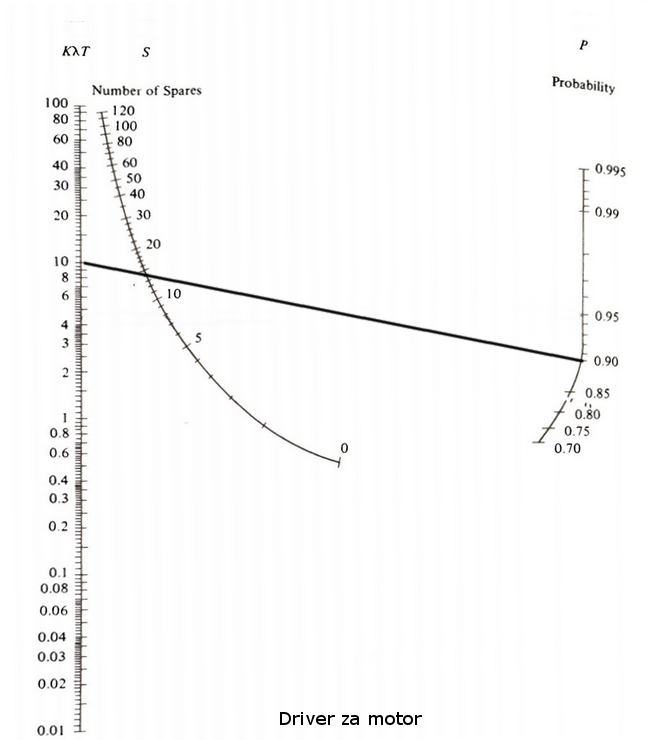
\includegraphics[scale=0.6]{driver_za_motore.png}
\caption{Grafički način određivanja broja potrebnog broja rezervnih komponenti}
\label{slika_rezerve}
\end{figure}

\begin{landscape}

% Table generated by Excel2LaTeX from sheet 'Broj rezervnih dijelova'
\begin{table}[htbp]
  \centering
  \caption{Potreban broj rezervnih dijelova za rješenja 1 i 2}
    \begin{tabular}{ccrrr}
    \multicolumn{5}{c}{Rješenje 1} \\
    \midrule
    Cjelina & Komponente & \multicolumn{1}{p{7.93em}}{Broj rezervnih \newline{}dijelova, 50 \newline{}jedinica godišnje} & \multicolumn{1}{p{8.285em}}{Broj rezervnih \newline{}dijelova, 100 \newline{}jedinica godišnje} & \multicolumn{1}{c}{Cijena (KM)} \\
    \midrule
    \multirow{2}[2]{*}{Upravljačka jedinica} & \multicolumn{1}{l}{Driver za motore} & 14    & 28    & 20 \\
          & \multicolumn{1}{l}{Mikrokontroler} & 14    & 28    & 10 \\
    \midrule
    \multirow{4}[2]{*}{Mehanizam printanja} & \multicolumn{1}{l}{Motori} & 28    & 55    & 250 \\
          & \multicolumn{1}{l}{Okvir} & 5     & 8     & 100 \\
          & \multicolumn{1}{l}{Prskalica} & 18    & 35    & 20 \\
          & \multicolumn{1}{l}{Spremnik pritiska} & 12    & 24    & 25 \\
    \midrule
    \multirow{2}[2]{*}{Komunikacija} & \multicolumn{1}{l}{Wifi modul za komunikaciju} & 17    & 35    & 5 \\
          & \multicolumn{1}{l}{USB modul za komunikaciju} & 17    & 35    & 5 \\
    \midrule
    \multicolumn{2}{c}{Cijena prve nabavke (KM):} & 8750  & 17040 &  \\
    \midrule
    \multicolumn{5}{c}{Rješenje 2} \\
    \midrule
    \multirow{2}[2]{*}{Upravljačka jedinica} & \multicolumn{1}{l}{Driver za motore} & 14    & 28    & 20 \\
          & \multicolumn{1}{l}{Mikrokontroler} & 14    & 28    & 10 \\
    \midrule
    \multirow{4}[2]{*}{Mehanizam printanja} & \multicolumn{1}{l}{Motori} & 28    & 55    & 250 \\
          & \multicolumn{1}{l}{Okvir} & 5     & 8     & 50 \\
          & \multicolumn{1}{l}{Prskalica} & 18    & 35    & 20 \\
          & \multicolumn{1}{l}{Spremnik pritiska} & 12    & 24    & 25 \\
    \midrule
    \multirow{2}[2]{*}{Komunikacija} & \multicolumn{1}{l}{Wifi modul za komunikaciju} & 17    & 35    & 5 \\
          & \multicolumn{1}{l}{USB modul za komunikaciju} & 17    & 35    & 5 \\
    \midrule
    \multicolumn{2}{c}{Cijena prve nabavke (KM):} & 8500  & 16640 &  \\
    \bottomrule
    \end{tabular}%
  \label{tab:rezerve1}%
\end{table}%

% Table generated by Excel2LaTeX from sheet 'Broj rezervnih dijelova'
\begin{table}[htbp]
  \centering
  \caption{Potreban broj rezervnih dijelova za rješenje 3}
    \begin{tabular}{ccrrr}
    \toprule
    Cjelina & Komponente & \multicolumn{1}{p{7.93em}}{Broj rezervnih \newline{}dijelova, 50 \newline{}jedinica godišnje} & \multicolumn{1}{p{8.285em}}{Broj rezervnih \newline{}dijelova, 100 \newline{}jedinica godišnje} & \multicolumn{1}{c}{Cijena (KM)} \\
    \midrule
    \multirow{2}[2]{*}{Upravljačka jedinica} & \multicolumn{1}{l}{Driver za motore} & 14    & 28    & 20 \\
          & \multicolumn{1}{l}{Mikrokontroler} & 14    & 28    & 10 \\
    \midrule
    \multirow{4}[2]{*}{Mehanizam printanja} & \multicolumn{1}{l}{Motori} & 50    & 80    & 150 \\
          & \multicolumn{1}{l}{Okvir} & 5     & 8     & 100 \\
          & \multicolumn{1}{l}{Prskalica} & 35    & 55    & 20 \\
          & \multicolumn{1}{l}{Spremnik pritiska} & 12    & 24    & 25 \\
    \midrule
    \multirow{2}[2]{*}{Komunikacija} & \multicolumn{1}{l}{Wifi modul za komunikaciju} & 17    & 35    & 5 \\
          & \multicolumn{1}{l}{USB modul za komunikaciju} & 17    & 35    & 5 \\
    \midrule
    \multicolumn{2}{c}{Cijena prve nabavke (KM):} & 9590  & 15690 &  \\
    \bottomrule
    \end{tabular}%
  \label{tab:rezerve2}%
\end{table}%

\end{landscape}
\subsection{Life-cycle cost analiza}
Kako bi se odredila profitabilnost projekta potrebno je utvrditi sve troškove i prihode. LCC anliza upravo služi za određivanje troškova tokom čitavog perioda proizvodnje i podrške. Uzeta su dva slučaja. U prvom slučaju se proizvodi 50 uređaja godišnje (slika \ref{plan50}), a u drugom 100 (slika \ref{plan100}). Proizvodnja traje 8 godina. Povećan broj uređaja znači i veći prihodi, međutim to povlači za sobom i veći broj jedinica za održavanje, tako da je moguće da će manji broj proizvedenih jedinica povećati profitabilnost. Rezultat analize se može vidjeti na tabelama \ref{rj1_50}, \ref{rj1_100}, \ref{rj2_50}, \ref{rj2_100}, \ref{rj3_50}, \ref{rj3_100}.



\begin{figure*}[ht!]
    \centering
    \begin{subfigure}[t]{0.45\textwidth}
		\centering
		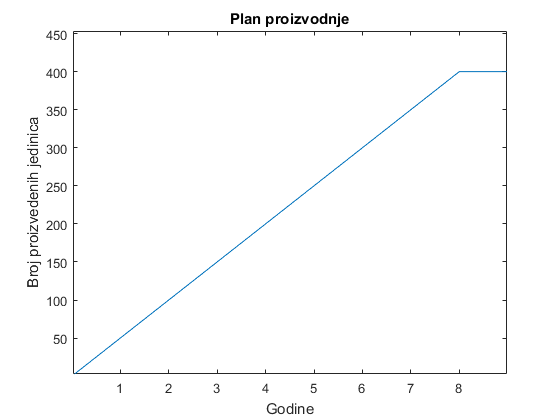
\includegraphics[scale = 0.45]{plan_proizvodnje/plan_proizvodnje-50}
		\caption{Ukupan broj proizvedenih jedinica kod proizvodnje 50 jedinica godišnje}
    \end{subfigure}%
    ~ 
    \begin{subfigure}[t]{0.45\textwidth}
		\centering
		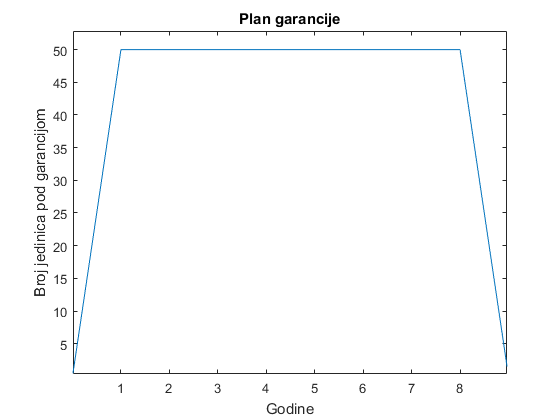
\includegraphics[scale = 0.45]{plan_proizvodnje/plan_garancije-50}
		\caption{Ukupan broj jedinica pod garancijom kod proizvodnje 50 jedinica godišnje}
    \end{subfigure}
    \caption{Plan proizvodnje i plan garancije za 50 jedinica proizvedenih godišnje}
    \label{plan50}
\end{figure*}

\begin{figure*}[ht!]
    \centering
    \begin{subfigure}[t]{0.45\textwidth}
		\centering
		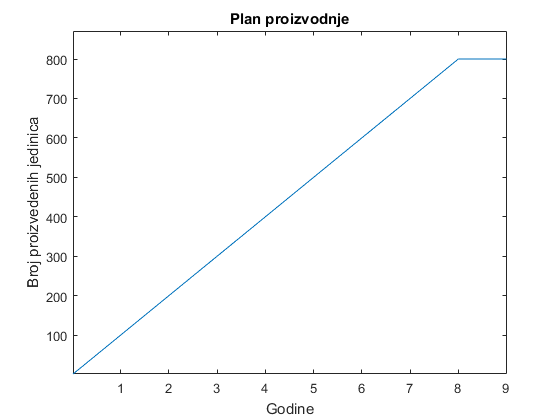
\includegraphics[scale = 0.45]{plan_proizvodnje/plan_proizvodnje-100}
		\caption{Ukupan broj proizvedenih jedinica kod proizvodnje 100 jedinica godišnje}
    \end{subfigure}%
    ~ 
    \begin{subfigure}[t]{0.45\textwidth}
		\centering
		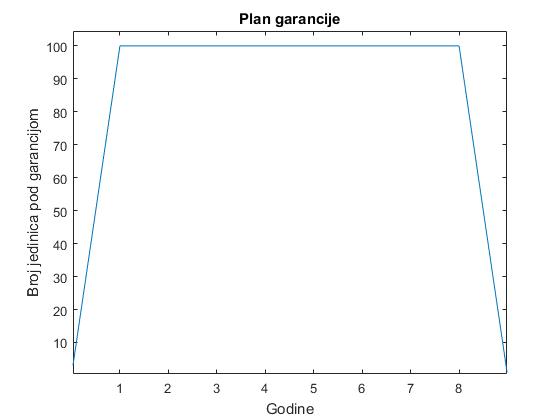
\includegraphics[scale = 0.45]{plan_proizvodnje/plan_garancije-100}
		\caption{Ukupan broj jedinica pod garancijom kod proizvodnje 100 jedinica godišnje}
    \end{subfigure}
    \caption{Plan proizvodnje i plan garancije za 100 jedinica proizvedenih godišnje}
    \label{plan100}
\end{figure*}
\clearpage

\begin{landscape}
% Table generated by Excel2LaTeX from sheet 'Life Cycle cost analiza'
\begin{table}[htbp]
  \centering
  \small
  \caption{Troškovi za rješenje 1, 50 jedinica proizvedeno godišnje}
    \begin{tabular}{lrrrrrrrrrr}
    \toprule
    \multicolumn{1}{c}{\multirow{2}[4]{*}{Aktivnost}} & \multicolumn{9}{c}{Cijena programa po godini}                         & \multicolumn{1}{c}{\multirow{2}[4]{*}{Total}} \\
\cmidrule{2-10}          & 1     & 2     & 3     & 4     & 5     & 6     & 7     & 8     & 9     &  \\
    \midrule
    \textbf{1. Istraživanje i razvoj} &       &       &       &       &       &       &       &       &       & 0 \\
    1.1. Dizajn za održivost & 500   & 500   &       &       &       &       &       &       &       & 1000 \\
    1.2. Dizajn za pouzdanost & 500   & 500   &       &       &       &       &       &       &       & 1000 \\
    1.3 Komponente za prvi prototip & 1000  &       &       &       &       &       &       &       &       & 1000 \\
    1.4 Software & 2000  & 2000  & 2000  & 2000  & 2000  & 2000  & 2000  & 2000  & 2000  & 18000 \\
    \midrule
    \textbf{Ukupno po katergoriji:} & 4000  & 3000  & 2000  & 2000  & 2000  & 2000  & 2000  & 2000  & 2000  & \textbf{21000} \\
    \midrule
    \textbf{2. Proizvodnja/konstrukcija} &       &       &       &       &       &       &       &       &       & 0 \\
    2.1 Iznajmljivanje prostora & 6000  & 6000  & 6000  & 6000  & 6000  & 6000  & 6000  & 6000  & 6000  & 54000 \\
    \multicolumn{1}{p{14.715em}}{2.2 Kupovina komponenti za\newline{}proizvodnju} & 21750 & 21750 & 21750 & 21750 & 21750 & 21750 & 21750 & 21750 & 0     & 174000 \\
    2.3 Kupovina opreme & 500   & 250   &       &       &       &       &       &       &       & 750 \\
    2.4 Slanje proizvoda & 2500  & 2500  & 2500  & 2500  & 2500  & 2500  & 2500  & 2500  & 0     & 20000 \\
    \midrule
    \textbf{Ukupno po kategoriji:} & 30750 & 30500 & 30250 & 30250 & 30250 & 30250 & 30250 & 30250 & 6000  & \textbf{248750} \\
    \midrule
    \textbf{3. Rad i podrška} &       &       &       &       &       &       &       &       &       & 0 \\
    3.1 Plate uposlenicima & 81600 & 81600 & 81600 & 81600 & 81600 & 81600 & 81600 & 81600 & 81600 & 734400 \\
    \multicolumn{1}{p{14.715em}}{3.2 Prva kupovina rezervnih\newline{} komponenti} & 8750  &       &       &       &       &       &       &       &       & 8750 \\
    3.3 Održavanje broja komponenti & 25500 & 25500 & 25500 & 25500 & 25500 & 25500 & 25500 & 25500 & 25500 & 229500 \\
    3.4. Održavanje vozila & 2400  & 2400  & 2400  & 2400  & 2400  & 2400  & 2400  & 2400  & 2400  & 21600 \\
    \midrule
    \textbf{Ukupno po kategoriji:} & 118250 & 109500 & 109500 & 109500 & 109500 & 109500 & 109500 & 109500 & 109500 & \textbf{994250} \\
    \midrule
    \textbf{Ukupno:} & 153000 & 143000 & 141750 & 141750 & 141750 & 141750 & 141750 & 141750 & 117500 & \textbf{1264000} \\

    \bottomrule
    \end{tabular}%
  \label{rj1_50}%
\end{table}%

\end{landscape}


\begin{landscape}
% Table generated by Excel2LaTeX from sheet 'Life Cycle cost analiza'
\begin{table}[htbp]
  \centering
  \small
  \caption{Troškovi za rješenje 1, 100 jedinica proizvedeno godišnje}
    \begin{tabular}{lrrrrrrrrrr}
    \toprule
    \multicolumn{1}{c}{\multirow{2}[4]{*}{Aktivnost}} & \multicolumn{9}{c}{Cijena programa po godini}                         & \multicolumn{1}{c}{\multirow{2}[4]{*}{Total}} \\
\cmidrule{2-10}          & 1     & 2     & 3     & 4     & 5     & 6     & 7     & 8     & 9     &  \\
    \midrule
    \textbf{1. Istraživanje i razvoj} &       &       &       &       &       &       &       &       &       & 0 \\
    1.1. Dizajn za održivost & 500   & 500   &       &       &       &       &       &       &       & 1000 \\
    1.2. Dizajn za pouzdanost & 500   & 500   &       &       &       &       &       &       &       & 1000 \\
    1.3 Komponente za prvi prototip & 1000  &       &       &       &       &       &       &       &       & 1000 \\
    1.4 Software & 2000  & 2000  & 2000  & 2000  & 2000  & 2000  & 2000  & 2000  & 2000  & 18000 \\
    \midrule
    \textbf{Ukupno po katergoriji:} & 4000  & 3000  & 2000  & 2000  & 2000  & 2000  & 2000  & 2000  & 2000  & \textbf{21000} \\
    \midrule
    \textbf{2. Proizvodnja/konstrukcija} &       &       &       &       &       &       &       &       &       & 0 \\
    2.1 Iznajmljivanje prostora & 6000  & 6000  & 6000  & 6000  & 6000  & 6000  & 6000  & 6000  & 6000  & 54000 \\
    \multicolumn{1}{p{14.715em}}{2.2 Kupovina komponenti za\newline{}proizvodnju} & 43500 & 43500 & 43500 & 43500 & 43500 & 43500 & 43500 & 43500 & 0     & 348000 \\
    2.3 Kupovina opreme & 500   & 250   &       &       &       &       &       &       &       & 750 \\
    2.4 Slanje proizvoda & 5000  & 5000  & 5000  & 5000  & 5000  & 5000  & 5000  & 5000  & 0     & 40000 \\
    \midrule
    \textbf{Ukupno po kategoriji:} & 55000 & 54750 & 54500 & 54500 & 54500 & 54500 & 54500 & 54500 & 6000  & \textbf{442750} \\
    \midrule
    \textbf{3. Rad i podrška} &       &       &       &       &       &       &       &       &       & 0 \\
    3.1 Plate uposlenicima & 81600 & 81600 & 81600 & 81600 & 81600 & 81600 & 81600 & 81600 & 81600 & 734400 \\
    \multicolumn{1}{p{14.715em}}{3.2 Prva kupovina rezervnih\newline{} komponenti} & 17040 &       &       &       &       &       &       &       &       & 17040 \\
    3.3 Održavanje broja komponenti & 51000 & 51000 & 51000 & 51000 & 51000 & 51000 & 51000 & 51000 & 51000 & 459000 \\
    3.4. Održavanje vozila & 2400  & 2400  & 2400  & 2400  & 2400  & 2400  & 2400  & 2400  & 2400  & 21600 \\
    \midrule
    \textbf{Ukupno po kategoriji:} & 152040 & 135000 & 135000 & 135000 & 135000 & 135000 & 135000 & 135000 & 135000 & \textbf{1232040} \\
    \midrule
    \textbf{Ukupno:} & 211040 & 192750 & 191500 & 191500 & 191500 & 191500 & 191500 & 191500 & 143000 & \textbf{1695790} \\

    \bottomrule
    \end{tabular}%
  \label{rj1_100}%
\end{table}%

\end{landscape}


\begin{landscape}
% Table generated by Excel2LaTeX from sheet 'Life Cycle cost analiza'
\begin{table}[htbp]
  \centering
  \small
  \caption{Troškovi za rješenje 2, 50 jedinica proizvedeno godišnje}
    \begin{tabular}{lrrrrrrrrrr}
    \toprule
    \multicolumn{1}{c}{\multirow{2}[4]{*}{Aktivnost}} & \multicolumn{9}{c}{Cijena programa po godini}                         & \multicolumn{1}{c}{\multirow{2}[4]{*}{Total}} \\
\cmidrule{2-10}          & 1     & 2     & 3     & 4     & 5     & 6     & 7     & 8     & 9     &  \\
    \midrule
\textbf{1. Istraživanje i razvoj} &       &       &       &       &       &       &       &       &       & 0 \\
    1.1. Dizajn za održivost & 500   & 500   &       &       &       &       &       &       &       & 1000 \\
    1.2. Dizajn za pouzdanost & 500   & 500   &       &       &       &       &       &       &       & 1000 \\
    1.3 Komponente za prvi prototip & 1000  &       &       &       &       &       &       &       &       & 1000 \\
    1.4 Software & 2000  & 2000  & 2000  & 2000  & 2000  & 2000  & 2000  & 2000  & 2000  & 18000 \\
    \midrule
    \textbf{Ukupno po katergoriji:} & 4000  & 3000  & 2000  & 2000  & 2000  & 2000  & 2000  & 2000  & 2000  & \textbf{21000} \\
    \midrule
    \textbf{2. Proizvodnja/konstrukcija} &       &       &       &       &       &       &       &       &       & 0 \\
    2.1 Iznajmljivanje prostora & 6000  & 6000  & 6000  & 6000  & 6000  & 6000  & 6000  & 6000  & 6000  & 54000 \\
    \multicolumn{1}{p{14.715em}}{2.2 Kupovina komponenti za\newline{}proizvodnju} & 19250 & 19250 & 19250 & 19250 & 19250 & 19250 & 19250 & 19250 & 0     & 154000 \\
    2.3 Kupovina opreme & 500   & 250   &       &       &       &       &       &       &       & 750 \\
    2.4 Slanje proizvoda & 2500  & 2500  & 2500  & 2500  & 2500  & 2500  & 2500  & 2500  & 0     & 20000 \\
    \midrule
    \textbf{Ukupno po kategoriji:} & 28250 & 28000 & 27750 & 27750 & 27750 & 27750 & 27750 & 27750 & 6000  & \textbf{228750} \\
    \midrule
    \textbf{3. Rad i podrška} &       &       &       &       &       &       &       &       &       & 0 \\
    3.1 Plate uposlenicima & 81600 & 81600 & 81600 & 81600 & 81600 & 81600 & 81600 & 81600 & 81600 & 734400 \\
    \multicolumn{1}{p{14.715em}}{3.2 Prva kupovina rezervnih\newline{} komponenti} & 8500  &       &       &       &       &       &       &       &       & 8500 \\
    3.3 Održavanje broja komponenti & 25000 & 25000 & 25000 & 25000 & 25000 & 25000 & 25000 & 25000 & 25000 & 225000 \\
    3.4. Održavanje vozila & 2400  & 2400  & 2400  & 2400  & 2400  & 2400  & 2400  & 2400  & 2400  & 21600 \\
    \midrule
    \textbf{Ukupno po kategoriji:} & 117500 & 109000 & 109000 & 109000 & 109000 & 109000 & 109000 & 109000 & 109000 & \textbf{989500} \\
    \midrule
    \textbf{Ukupno:} & 149750 & 140000 & 138750 & 138750 & 138750 & 138750 & 138750 & 138750 & 117000 & \textbf{1239250} \\

    \bottomrule
    \end{tabular}%
  \label{rj2_50}%
\end{table}%

\end{landscape}


\begin{landscape}
% Table generated by Excel2LaTeX from sheet 'Life Cycle cost analiza'
\begin{table}[htbp]
  \centering
  \small
  \caption{Troškovi za rješenje 2, 100 jedinica proizvedeno godišnje}
    \begin{tabular}{lrrrrrrrrrr}
    \toprule
    \multicolumn{1}{c}{\multirow{2}[4]{*}{Aktivnost}} & \multicolumn{9}{c}{Cijena programa po godini}                         & \multicolumn{1}{c}{\multirow{2}[4]{*}{Total}} \\
\cmidrule{2-10}          & 1     & 2     & 3     & 4     & 5     & 6     & 7     & 8     & 9     &  \\
    \midrule
    \textbf{1. Istraživanje i razvoj} &       &       &       &       &       &       &       &       &       & 0 \\
    1.1. Dizajn za održivost & 500   & 500   &       &       &       &       &       &       &       & 1000 \\
    1.2. Dizajn za pouzdanost & 500   & 500   &       &       &       &       &       &       &       & 1000 \\
    1.3 Komponente za prvi prototip & 1000  &       &       &       &       &       &       &       &       & 1000 \\
    1.4 Software & 2000  & 2000  & 2000  & 2000  & 2000  & 2000  & 2000  & 2000  & 2000  & 18000 \\
    \midrule
    \textbf{Ukupno po katergoriji:} & 4000  & 3000  & 2000  & 2000  & 2000  & 2000  & 2000  & 2000  & 2000  & \textbf{21000} \\
    \midrule
    \textbf{2. Proizvodnja/konstrukcija} &       &       &       &       &       &       &       &       &       & 0 \\
    2.1 Iznajmljivanje prostora & 6000  & 6000  & 6000  & 6000  & 6000  & 6000  & 6000  & 6000  & 6000  & 54000 \\
    \multicolumn{1}{p{14.715em}}{2.2 Kupovina komponenti za\newline{}proizvodnju} & 38500 & 19250 & 19250 & 19250 & 19250 & 19250 & 19250 & 19250 & 0     & 173250 \\
    2.3 Kupovina opreme & 500   & 250   &       &       &       &       &       &       &       & 750 \\
    2.4 Slanje proizvoda & 5000  & 5000  & 5000  & 5000  & 5000  & 5000  & 5000  & 5000  & 5000  & 45000 \\
    \midrule
    \textbf{Ukupno po kategoriji:} & 50000 & 30500 & 30250 & 30250 & 30250 & 30250 & 30250 & 30250 & 11000 & \textbf{273000} \\
    \midrule
    \textbf{3. Rad i podrška} &       &       &       &       &       &       &       &       &       & 0 \\
    3.1 Plate uposlenicima & 81600 & 81600 & 81600 & 81600 & 81600 & 81600 & 81600 & 81600 & 81600 & 734400 \\
    \multicolumn{1}{p{14.715em}}{3.2 Prva kupovina rezervnih\newline{} komponenti} & 16640 &       &       &       &       &       &       &       &       & 16640 \\
    3.3 Održavanje broja komponenti & 50000 & 50000 & 50000 & 50000 & 50000 & 50000 & 50000 & 50000 & 50000 & 450000 \\
    3.4. Održavanje vozila & 2400  & 2400  & 2400  & 2400  & 2400  & 2400  & 2400  & 2400  & 2400  & 21600 \\
    \midrule
    \textbf{Ukupno po kategoriji:} & 150640 & 134000 & 134000 & 134000 & 134000 & 134000 & 134000 & 134000 & 134000 & \textbf{1222640} \\
    \midrule
    \textbf{Ukupno:} & 204640 & 167500 & 166250 & 166250 & 166250 & 166250 & 166250 & 166250 & 147000 & \textbf{1516640} \\

    \bottomrule
    \end{tabular}%
  \label{rj2_100}%
\end{table}%

\end{landscape}


\begin{landscape}
% Table generated by Excel2LaTeX from sheet 'Life Cycle cost analiza'
\begin{table}[htbp]
  \centering
  \small
  \caption{Troškovi za rješenje 3, 50 jedinica proizvedeno godišnje}
    \begin{tabular}{lrrrrrrrrrr}
    \toprule
    \multicolumn{1}{c}{\multirow{2}[4]{*}{Aktivnost}} & \multicolumn{9}{c}{Cijena programa po godini}                         & \multicolumn{1}{c}{\multirow{2}[4]{*}{Total}} \\
\cmidrule{2-10}          & 1     & 2     & 3     & 4     & 5     & 6     & 7     & 8     & 9     &  \\
    \midrule
    \textbf{1. Istraživanje i razvoj} &       &       &       &       &       &       &       &       &       & 0 \\
    1.1. Dizajn za održivost & 500   & 500   &       &       &       &       &       &       &       & 1000 \\
    1.2. Dizajn za pouzdanost & 500   & 500   &       &       &       &       &       &       &       & 1000 \\
    1.3 Komponente za prvi prototip & 1000  &       &       &       &       &       &       &       &       & 1000 \\
    1.4 Software & 2000  & 2000  & 2000  & 2000  & 2000  & 2000  & 2000  & 2000  & 2000  & 18000 \\
    \midrule
    \textbf{Ukupno po katergoriji:} & 4000  & 3000  & 2000  & 2000  & 2000  & 2000  & 2000  & 2000  & 2000  & \textbf{21000} \\
    \midrule
    \textbf{2. Proizvodnja/konstrukcija} &       &       &       &       &       &       &       &       &       & 0 \\
    2.1 Iznajmljivanje prostora & 6000  & 6000  & 6000  & 6000  & 6000  & 6000  & 6000  & 6000  & 6000  & 54000 \\
    \multicolumn{1}{p{14.715em}}{2.2 Kupovina komponenti za\newline{}proizvodnju} & 16750 & 16750 & 16750 & 16750 & 16750 & 16750 & 16750 & 16750 & 0     & 134000 \\
    2.3 Kupovina opreme & 500   & 250   &       &       &       &       &       &       &       & 750 \\
    2.4 Slanje proizvoda & 2500  & 2500  & 2500  & 2500  & 2500  & 2500  & 2500  & 2500  & 0     & 20000 \\
    \midrule
    \textbf{Ukupno po kategoriji:} & 25750 & 25500 & 25250 & 25250 & 25250 & 25250 & 25250 & 25250 & 6000  & \textbf{208750} \\
    \midrule
    \textbf{3. Rad i podrška} &       &       &       &       &       &       &       &       &       & 0 \\
    3.1 Plate uposlenicima & 81600 & 81600 & 81600 & 81600 & 81600 & 81600 & 81600 & 81600 & 81600 & 734400 \\
    \multicolumn{1}{p{14.715em}}{3.2 Prva kupovina rezervnih\newline{} komponenti} & 9590  &       &       &       &       &       &       &       &       & 9590 \\
    3.3 Održavanje broja komponenti & 30700 & 30700 & 30700 & 30700 & 30700 & 30700 & 30700 & 30700 & 30700 & 276300 \\
    3.4. Održavanje vozila & 2400  & 2400  & 2400  & 2400  & 2400  & 2400  & 2400  & 2400  & 2400  & 21600 \\
    \midrule
    \textbf{Ukupno po kategoriji:} & 124290 & 114700 & 114700 & 114700 & 114700 & 114700 & 114700 & 114700 & 114700 & \textbf{1041890} \\
    \midrule
    \textbf{Ukupno:} & 154040 & 143200 & 141950 & 141950 & 141950 & 141950 & 141950 & 141950 & 122700 & \textbf{1271640} \\

    \bottomrule
    \end{tabular}%
  \label{rj3_50}%
\end{table}%

\end{landscape}

\begin{landscape}
% Table generated by Excel2LaTeX from sheet 'Life Cycle cost analiza'
\begin{table}[htbp]
  \centering
  \small
  \caption{Troškovi za rješenje 3, 100 jedinica proizvedeno godišnje}
    \begin{tabular}{lrrrrrrrrrr}
    \toprule
    \multicolumn{1}{c}{\multirow{2}[4]{*}{Aktivnost}} & \multicolumn{9}{c}{Cijena programa po godini}                         & \multicolumn{1}{c}{\multirow{2}[4]{*}{Total}} \\
\cmidrule{2-10}          & 1     & 2     & 3     & 4     & 5     & 6     & 7     & 8     & 9     &  \\
    \midrule
\textbf{1. Istraživanje i razvoj} &       &       &       &       &       &       &       &       &       & 0 \\
    1.1. Dizajn za održivost & 500   & 500   &       &       &       &       &       &       &       & 1000 \\
    1.2. Dizajn za pouzdanost & 500   & 500   &       &       &       &       &       &       &       & 1000 \\
    1.3 Komponente za prvi prototip & 1000  &       &       &       &       &       &       &       &       & 1000 \\
    1.4 Software & 2000  & 2000  & 2000  & 2000  & 2000  & 2000  & 2000  & 2000  & 2000  & 18000 \\
    \midrule
    \textbf{Ukupno po katergoriji:} & 4000  & 3000  & 2000  & 2000  & 2000  & 2000  & 2000  & 2000  & 2000  & \textbf{21000} \\
    \midrule
    \textbf{2. Proizvodnja/konstrukcija} &       &       &       &       &       &       &       &       &       & 0 \\
    2.1 Iznajmljivanje prostora & 6000  & 6000  & 6000  & 6000  & 6000  & 6000  & 6000  & 6000  & 6000  & 54000 \\
    \multicolumn{1}{p{14.715em}}{2.2 Kupovina komponenti za\newline{}proizvodnju} & 33500 & 33500 & 33500 & 33500 & 33500 & 33500 & 33500 & 33500 & 0     & 268000 \\
    2.3 Kupovina opreme & 500   & 250   &       &       &       &       &       &       &       & 750 \\
    2.4 Slanje proizvoda & 5000  & 5000  & 5000  & 5000  & 5000  & 5000  & 5000  & 5000  & 0     & 40000 \\
    \midrule
    \textbf{Ukupno po kategoriji:} & 45000 & 44750 & 44500 & 44500 & 44500 & 44500 & 44500 & 44500 & 6000  & \textbf{362750} \\
    \midrule
    \textbf{3. Rad i podrška} &       &       &       &       &       &       &       &       &       & 0 \\
    3.1 Plate uposlenicima & 81600 & 81600 & 81600 & 81600 & 81600 & 81600 & 81600 & 81600 & 81600 & 734400 \\
    \multicolumn{1}{p{14.715em}}{3.2 Prva kupovina rezervnih\newline{} komponenti} & 15690 &       &       &       &       &       &       &       &       & 15690 \\
    3.3 Održavanje broja komponenti & 61400 & 61400 & 61400 & 61400 & 61400 & 61400 & 61400 & 61400 & 61400 & 552600 \\
    3.4. Održavanje vozila & 2400  & 2400  & 2400  & 2400  & 2400  & 2400  & 2400  & 2400  & 2400  & 21600 \\
    \midrule
    \textbf{Ukupno po kategoriji:} & 161090 & 145400 & 145400 & 145400 & 145400 & 145400 & 145400 & 145400 & 145400 & \textbf{1324290} \\
    \midrule
    \textbf{Ukupno:} & 210090 & 193150 & 191900 & 191900 & 191900 & 191900 & 191900 & 191900 & 153400 & \textbf{1708040} \\

    \bottomrule
    \end{tabular}%
  \label{rj3_100}%
\end{table}%
\end{landscape}

\subsection{Analiza profitabilnosti}
Na osnovu svih prijašnjih analiza na kraju je moguće ustanoviti profitabilnost projekta. Kao što je viđeno u prijašnjim poglavljima, za svako rješenje je rađena analiza za slučaj proizvodnje 50 i za slučaj proizvodnje 100 jedinica godišnje. 

U analizi profitabilnosti je korištena vrijednost diskontnog faktora od 7\%. Jedina nepoznanica ostaje određivanje cijene konačnog proizvoda. Pošto je minimalna cijena također jedan od zahtjeva, za svaki od 6 različitih slučajeva je cijena iterativno povećevana za 500 KM sve dok na krajnjem rasponu od 9 godina ne bi ostvarili profit. Rezultat te analize se može vidjeti na tabelama \ref{profit1}, \ref{profit2} i \ref{profit3}.

Mogu se donijeti sljedeći zaključci
\begin{itemize}
\item Cijena uređaja za slučaj proizvodnje 50 jedinica je 3500 KM kod svakog rješenja
\item Cijena uređaja za slučaj proizvodnje 100 jedinica je 2500 KM kod svakog rješenja
\item Proizvodnja većeg broja uređaja je u svakom slučaju profitabilnija
\item Rješenje 2 je najprofitabilnije od svih rješenja.
\item Mada je rješenje 3 jeftinije za proizvodnju od rješenja 2, cijena vezana za pouzdanost i održavanje manje pouzdanih komponenti je više nego nadoknadila razliku
\item Ni jedno rješenje nije jeftinije od konkurentskog rješenja
\end{itemize}


\begin{landscape}
% Table generated by Excel2LaTeX from sheet 'LCC analiza 2'
\begin{table}[htbp]
  \centering
  \caption{Rješenje 1 - cashflow}
    \begin{tabular}{rrrrrrr}
    \toprule
    \multicolumn{1}{c}{Godina} & \multicolumn{1}{c}{Prihodi} & \multicolumn{1}{c}{Troškovi} & \multicolumn{1}{c}{Priliv novca} & \multicolumn{1}{c}{Diskontni faktor} & \multicolumn{1}{p{9.355em}}{Stvarna vrijednost \newline{}priliva novca} & \multicolumn{1}{c}{NPV} \\
    \midrule
          & \multicolumn{1}{c}{Investicija:} & \multicolumn{1}{c}{100000} & \multicolumn{1}{c}{Broj proizvedenih:} & \multicolumn{1}{c}{50} & \multicolumn{1}{c}{Cijena:} & \multicolumn{1}{c}{3000} \\
    \midrule
0     & 0     & -100000 & -100000 & 1     & -100000 & -100000 \\
    1     & 175000 & -153000 & 22000 & 0.934579439 & 20560.74766 & -79439.3 \\
    2     & 175000 & -143000 & 32000 & 0.873438728 & 27950.0393 & -51489.2 \\
    3     & 175000 & -141750 & 33250 & 0.816297877 & 27141.90441 & -24347.3 \\
    4     & 175000 & -141750 & 33250 & 0.762895212 & 25366.2658 & {\textbf{1018.957}} \\
    5     & 175000 & -141750 & 33250 & 0.712986179 & 23706.79047 & {\textbf{24725.75}} \\
    6     & 175000 & -141750 & 33250 & 0.666342224 & 22155.87894 & {\textbf{46881.63}} \\
    7     & 175000 & -141750 & 33250 & 0.622749742 & 20706.42892 & {\textbf{67588.06}} \\
    8     & 175000 & -141750 & 33250 & 0.582009105 & 19351.80273 & {\textbf{86939.86}} \\
    \midrule
    9     & 0     & -117500 & -117500 & 0.543933743 & -63912.21475 & \textbf{23027.64} \\
    \midrule
          & \multicolumn{1}{c}{Investicija:} & \multicolumn{1}{c}{100000} & \multicolumn{1}{c}{Broj proizvedenih:} & \multicolumn{1}{c}{100} & \multicolumn{1}{c}{Cijena:} & \multicolumn{1}{c}{2500} \\
    \midrule
    0     & 0     & -100000 & -100000 & 1     & -100000 & -100000 \\
    1     & 250000 & -211040 & 38960 & 0.934579439 & 36411.21495 & -63588.8 \\
    2     & 250000 & -192750 & 57250 & 0.873438728 & 50004.36719 & -13584.4 \\
    3     & 250000 & -191500 & 58500 & 0.816297877 & 47753.4258 & \textbf{34169.01} \\
    4     & 250000 & -191500 & 58500 & 0.762895212 & 44629.3699 & \textbf{78798.38} \\
    5     & 250000 & -191500 & 58500 & 0.712986179 & 41709.6915 & \textbf{120508.1} \\
    6     & 250000 & -191500 & 58500 & 0.666342224 & 38981.02009 & \textbf{159489.1} \\
    7     & 250000 & -191500 & 58500 & 0.622749742 & 36430.8599 & \textbf{195919.9} \\
    8     & 250000 & -191500 & 58500 & 0.582009105 & 34047.53262 & \textbf{229967.5} \\
    \midrule
    9     & 0     & -143000 & -143000 & 0.543933743 & -77782.52519 & \textbf{152185} \\
  
    \bottomrule
    \end{tabular}%
  \label{profit1}%
\end{table}%

\end{landscape}

\begin{landscape}
% Table generated by Excel2LaTeX from sheet 'LCC analiza 2'
\begin{table}[htbp]
  \centering
  \caption{Rješenje 2 - cashflow}
    \begin{tabular}{rrrrrrr}
    \toprule
    \multicolumn{1}{c}{Godina} & \multicolumn{1}{c}{Prihodi} & \multicolumn{1}{c}{Troškovi} & \multicolumn{1}{c}{Priliv novca} & \multicolumn{1}{c}{Diskontni faktor} & \multicolumn{1}{p{8.145em}}{Stvarna vrijednost \newline{}priliva novca} & \multicolumn{1}{c}{NPV} \\
    \midrule
          & \multicolumn{1}{c}{Investicija:} & \multicolumn{1}{c}{100000} & \multicolumn{1}{c}{Broj proizvedenih:} & \multicolumn{1}{c}{50} & \multicolumn{1}{c}{Cijena:} & \multicolumn{1}{c}{3500} \\
    \midrule
0     & 0     & -100000 & -100000 & 1     & -100000 & -100000 \\
    1     & 175000 & -149750 & 25250 & 0.934579439 & 23598.13084 & -76401.9 \\
    2     & 175000 & -140000 & 35000 & 0.873438728 & 30570.35549 & -45831.5 \\
    3     & 175000 & -138750 & 36250 & 0.816297877 & 29590.79804 & -16240.7 \\
    4     & 175000 & -138750 & 36250 & 0.762895212 & 27654.95144 & \textbf{11414.24} \\
    5     & 175000 & -138750 & 36250 & 0.712986179 & 25845.74901 & \textbf{37259.98} \\
    6     & 175000 & -138750 & 36250 & 0.666342224 & 24154.90561 & \textbf{61414.89} \\
    7     & 175000 & -138750 & 36250 & 0.622749742 & 22574.67814 & \textbf{83989.57} \\
    8     & 175000 & -138750 & 36250 & 0.582009105 & 21097.83004 & \textbf{105087.4} \\
    \midrule
    9     & 0     & -117000 & -117000 & 0.543933743 & -63640.24788 & \textbf{41447.15} \\
    \midrule
          & \multicolumn{1}{c}{Investicija:} & \multicolumn{1}{c}{100000} & \multicolumn{1}{c}{Broj proizvedenih:} & \multicolumn{1}{c}{100} & \multicolumn{1}{c}{Cijena:} & \multicolumn{1}{c}{2500} \\
    \midrule
    0     & 0     & -100000 & -100000 & 1     & -100000 & -100000 \\
    1     & 250000 & -204640 & 45360 & 0.934579439 & 42392.52336 & -57607.5 \\
    2     & 250000 & -167500 & 82500 & 0.873438728 & 72058.69508 & \textbf{14451.22} \\
    3     & 250000 & -166250 & 83750 & 0.816297877 & 68364.94719 & \textbf{82816.17} \\
    4     & 250000 & -166250 & 83750 & 0.762895212 & 63892.47401 & \textbf{146708.6} \\
    5     & 250000 & -166250 & 83750 & 0.712986179 & 59712.59253 & \textbf{206421.2} \\
    6     & 250000 & -166250 & 83750 & 0.666342224 & 55806.16124 & \textbf{262227.4} \\
    7     & 250000 & -166250 & 83750 & 0.622749742 & 52155.29088 & \textbf{314382.7} \\
    8     & 250000 & -166250 & 83750 & 0.582009105 & 48743.26251 & \textbf{363125.9} \\
    \midrule
    9     & 0     & -147000 & -147000 & 0.543933743 & -79958.26016 & \textbf{283167.7} \\
    
    \bottomrule
    \end{tabular}%
  \label{profit2}%
\end{table}%
\end{landscape}

\begin{landscape}
% Table generated by Excel2LaTeX from sheet 'LCC analiza 2'
\begin{table}[htbp]
  \centering
  \caption{Rješenje 3 - cashflow}
    \begin{tabular}{rrrrrrr}
    \toprule
    \multicolumn{1}{c}{Godina} & \multicolumn{1}{c}{Prihodi} & \multicolumn{1}{c}{Troškovi} & \multicolumn{1}{c}{Priliv novca} & \multicolumn{1}{c}{Diskontni faktor} & \multicolumn{1}{p{8.145em}}{Stvarna vrijednost \newline{}priliva novca} & \multicolumn{1}{c}{NPV} \\
    \midrule
          & \multicolumn{1}{c}{Investicija:} & \multicolumn{1}{c}{100000} & \multicolumn{1}{c}{Broj proizvedenih:} & \multicolumn{1}{c}{50} & \multicolumn{1}{c}{Cijena:} & \multicolumn{1}{c}{3500} \\
    \midrule
0     & 0     & -100000 & -100000 & 1     & -100000 & -100000 \\
    1     & 175000 & -154040 & 20960 & 0.934579439 & 19588.78505 & -80411.2 \\
    2     & 175000 & -143200 & 31800 & 0.873438728 & 27775.35156 & -52635.9 \\
    3     & 175000 & -141950 & 33050 & 0.816297877 & 26978.64483 & -25657.2 \\
    4     & 175000 & -141950 & 33050 & 0.762895212 & 25213.68676 & -443.532 \\
    5     & 175000 & -141950 & 33050 & 0.712986179 & 23564.19323 & \textbf{23120.66} \\
    6     & 175000 & -141950 & 33050 & 0.666342224 & 22022.6105 & \textbf{45143.27} \\
    7     & 175000 & -141950 & 33050 & 0.622749742 & 20581.87897 & \textbf{65725.15} \\
    8     & 175000 & -141950 & 33050 & 0.582009105 & 19235.40091 & \textbf{84960.55} \\
    \midrule
    9     & 0     & -122700 & -122700 & 0.543933743 & -66740.67022 & \textbf{18219.88} \\
    \midrule
          & \multicolumn{1}{c}{Investicija:} & \multicolumn{1}{c}{100000} & \multicolumn{1}{c}{Broj proizvedenih:} & \multicolumn{1}{c}{100} & \multicolumn{1}{c}{Cijena:} & \multicolumn{1}{c}{2500} \\
    \midrule
    0     & 0     & -100000 & -100000 & 1     & -100000 & -100000 \\
    1     & 250000 & -210090 & 39910 & 0.934579439 & 37299.06542 & -62700.9 \\
    2     & 250000 & -193150 & 56850 & 0.873438728 & 49654.9917 & -13045.9 \\
    3     & 250000 & -191900 & 58100 & 0.816297877 & 47426.90665 & \textbf{34380.96} \\
    4     & 250000 & -191900 & 58100 & 0.762895212 & 44324.21182 & \textbf{78705.18} \\
    5     & 250000 & -191900 & 58100 & 0.712986179 & 41424.49703 & \textbf{120129.7} \\
    6     & 250000 & -191900 & 58100 & 0.666342224 & 38714.4832 & \textbf{158844.2} \\
    7     & 250000 & -191900 & 58100 & 0.622749742 & 36181.76 & \textbf{195025.9} \\
    8     & 250000 & -191900 & 58100 & 0.582009105 & 33814.72898 & \textbf{228840.6} \\
    \midrule
    9     & 0     & -153400 & -153400 & 0.543933743 & -83439.43611 & \textbf{145401.2} \\
    \bottomrule
    \end{tabular}%
  \label{profit3}%
\end{table}%

\end{landscape}

\section{Zaključak}

\bibliographystyle{unsrt}
\bibliography{mybib}

\end{document}
%modifikovao suad              
            

